% =====================================================================
%  HATI v2.0 -- Athena (IM-2) pre-landing hazard re-analysis
%  Author: Gergő Csaba Morvai
%  Engine: LuaLaTeX  (compile: latexmk -lualatex athena_paper.tex)
%  Bibliography: biblatex + biber
% =====================================================================
\documentclass[11pt]{article}

\usepackage{fontspec}
\usepackage{microtype}
\usepackage[a4paper,margin=2.45cm]{geometry}
\usepackage{graphicx}
\graphicspath{{../output/athena/}{../data/lroc_published/}{../output/}}
\usepackage{amsmath,amssymb}
\usepackage{xcolor}
\usepackage{booktabs}
\usepackage{array}
\usepackage{siunitx}
\usepackage[font=small]{caption}
\usepackage{enumitem}
\usepackage{tikz}
\usetikzlibrary{positioning,arrows.meta,calc,shapes.geometric,backgrounds,fit,decorations.pathmorphing}
\usepackage{tcolorbox}
\tcbuselibrary{skins,breakable}
\usepackage{titlesec}
\usepackage[backend=biber,style=authoryear,sorting=nyt,maxcitenames=2,uniquelist=false]{biblatex}
\addbibresource{references.bib}
\usepackage[hidelinks]{hyperref}
\usepackage{cleveref}

% ---- fonts (Palatino-style body, Helvetica-style sans, mono) ----
\setmainfont{TeX Gyre Pagella}
\setsansfont{TeX Gyre Heros}[Scale=0.92]
\setmonofont{TeX Gyre Cursor}[Scale=0.90]

% ---- palette ----
\definecolor{hatiblue}{HTML}{1F3A5F}
\definecolor{hatiaccent}{HTML}{B23A2E}
\definecolor{hatiteal}{HTML}{1B7A6E}
\definecolor{hatipurple}{HTML}{5B4B8A}
\definecolor{plainbg}{HTML}{EAF2FB}
\definecolor{plainframe}{HTML}{2E6DB4}
\definecolor{intentbg}{HTML}{F0EEF6}
\definecolor{intentframe}{HTML}{5B4B8A}
\definecolor{limitbg}{HTML}{FBEEEC}
\definecolor{limitframe}{HTML}{B23A2E}

% ---- headings ----
\titleformat{\section}{\sffamily\Large\bfseries\color{hatiblue}}{\thesection}{0.6em}{}
\titleformat{\subsection}{\sffamily\large\bfseries\color{hatiblue!88}}{\thesubsection}{0.5em}{}
\titleformat{\subsubsection}{\sffamily\normalsize\bfseries\color{hatiaccent}}{}{0em}{}
\titlespacing*{\section}{0pt}{1.6ex plus .3ex}{0.8ex}

% ---- callout boxes ----
\newtcolorbox{plainbox}{breakable,enhanced,colback=plainbg,colframe=plainframe,
  boxrule=0.6pt,arc=2pt,left=7pt,right=7pt,top=4pt,bottom=4pt,
  fonttitle=\bfseries\sffamily\small,coltitle=plainframe,
  attach boxed title to top left={xshift=8pt,yshift=-7pt},
  boxed title style={colback=plainbg,colframe=plainframe,boxrule=0.4pt,arc=1pt},
  title={In plain words}}
\newtcolorbox{intentbox}{breakable,enhanced,colback=intentbg,colframe=intentframe,
  boxrule=0.6pt,arc=2pt,left=7pt,right=7pt,top=4pt,bottom=4pt,
  fonttitle=\bfseries\sffamily\small,coltitle=intentframe,
  attach boxed title to top left={xshift=8pt,yshift=-7pt},
  boxed title style={colback=intentbg,colframe=intentframe,boxrule=0.4pt,arc=1pt},
  title={Why it is built this way}}
\newtcolorbox{limitbox}{breakable,enhanced,colback=limitbg,colframe=limitframe,
  boxrule=0.6pt,arc=2pt,left=7pt,right=7pt,top=4pt,bottom=4pt,
  fonttitle=\bfseries\sffamily\small,coltitle=limitframe,
  attach boxed title to top left={xshift=8pt,yshift=-7pt},
  boxed title style={colback=limitbg,colframe=limitframe,boxrule=0.4pt,arc=1pt},
  title={Honest limit}}

% ---- tikz styles ----
\tikzset{
  io/.style={rounded corners=3pt, draw=hatiblue, fill=hatiblue!8, align=center,
             inner sep=4pt, font=\footnotesize\sffamily, minimum height=9mm, text width=27mm},
  proc/.style={draw=black!55, fill=black!4, align=center, inner sep=4pt,
               font=\footnotesize\sffamily, minimum height=9mm, text width=30mm},
  dec/.style={diamond, draw=hatiaccent, fill=hatiaccent!12, align=center,
              font=\footnotesize\sffamily, inner sep=1pt, aspect=2.1, text width=17mm},
  flowarr/.style={-{Stealth[length=2.4mm]}, semithick, draw=black!65},
}

\sisetup{detect-all,per-mode=symbol}
\DeclareSIUnit{\px}{px}
\setlist{nosep,leftmargin=1.4em}
\captionsetup{labelfont={bf,sf,color=hatiblue}}

% =====================================================================
\title{\sffamily\bfseries\color{hatiblue}\LARGE HATI v2.0: a physics-based, two-channel\\ pipeline for lunar terrain-hazard detection\\[4pt]
\Large\mdseries Architecture, a forensic test on the IM-2 ``Athena'' loss,\\ and a resolution-ladder validation}
\author{\large Gergő Csaba Morvai\\[2pt]
\normalsize\itshape HATI v2.0 \textendash{} M\'ani Mission terrain-hazard pipeline}
\date{\normalsize June 2026}

\begin{document}
\maketitle

\begin{tcolorbox}[colback=limitbg,colframe=limitframe,boxrule=0.9pt,arc=2pt,
  left=8pt,right=8pt,top=6pt,bottom=6pt,fonttitle=\bfseries\sffamily\small,
  coltitle=limitframe,attach boxed title to top left={xshift=8pt,yshift=-7pt},
  boxed title style={colback=limitbg,colframe=limitframe,boxrule=0.4pt,arc=1pt},
  title={Superseded in part, June 2026}]
\small
This paper describes the v2.0 architecture as it stood when written, including a ten-descriptor
roughness heatmap. A later controlled cross-site experiment showed that eight of those ten
descriptors score \emph{below chance} when moved between sites (AUC $0.342$ to $0.432$: they rank
smooth ground above rough ground more often than not). Only RMS slope ($0.826$) and the terrain
ruggedness index ($0.808$) transfer. Those eight descriptors have been removed from the
operational pipeline, which is now two channels: a physical gross-terrain gate and the
sub-resolution shadow channel. The architecture, the fusion mathematics and the Athena forensic
work below all stand; the claim that the full texture stack is diagnostic does not. See the
status-and-roadmap report and \texttt{scripts/mare\_control\_v3.py} for the experiment and its
numbers.
\end{tcolorbox}
\medskip

\begin{abstract}
\noindent
Landing on the Moon means avoiding hazards smaller than the maps used to plan the
descent can resolve. We present HATI v2.0, a terrain-hazard pipeline built from two
physics-based, interpretable, training-free channels: a multi-scale roughness
\emph{heatmap} from a stereo elevation model, and a \emph{shadow census} that recovers
individual obstacles from a finer photograph, below the elevation model's resolution
floor. We define both channels in full, show that the fusion step is exactly a logistic
generalized linear model whose every weight has a stateable reason, and that the score
decomposes into exact per-channel contributions --- so each flag is auditable, the
property a flight system needs. We then do two things with the architecture. First, a
\emph{forensic test}: run the whole pipeline on the 2025 IM-2 ``Athena'' loss using only
pre-landing (2012) LROC data. The heatmap ranks the actual touchdown in the worst
\SI{3.7}{\percent} of an already-rough massif (robust $z=3.22$) on texture, not slope
(the local tilt is a gentle \ang{2.8}); the shadow census finds $\sim$\num{1400}
sub-resolution obstacles per \si{\kilo\meter\squared} the elevation model cannot see.
Second, a \emph{validation}: a resolution ladder that degrades real data and measures
how well each channel recovers the hazards visible at full resolution --- HATI's first
measured detection numbers. The shadow channel holds an AUC of $0.83$--$0.99$ with a
quantified size-reach; the heatmap recovers fine-data hazards from coarse elevation
models at AUC $0.86$--$0.93$. We state plainly what each result does and does not
establish, and fence what remains. The case for HATI is not that it is the most accurate
detector imaginable, but that it is an interpretable, certifiable one whose every number
traces back to physics.
\end{abstract}

\noindent\textbf{\sffamily\color{hatiblue}Keywords:}\enspace lunar landing hazards;
sub-resolution roughness; LROC NAC; shadow photoclinometry; Mons Mouton; terrain-relative navigation.

\medskip
\hrule
\medskip

% =====================================================================
\section{Introduction}

On 6 March 2025 the IM-2 spacecraft set down at roughly \ang{84.79}\,S,
\ang{29.20}\,E on Mons Mouton, deep in the lunar south-polar highlands, and tipped
over. The Lunar Reconnaissance Orbiter Camera (LROC) team later tied the upset to a
crater about \SI{20}{\meter} across sitting on sloped ground at the touchdown.

That is the hindsight story. This paper asks a different, harder question, and tries
to answer it without cheating: \emph{if we had run a dedicated terrain-hazard
analysis on the maps that already existed before the landing, would it have pointed
at that exact spot?}

\begin{figure}[t]
\centering
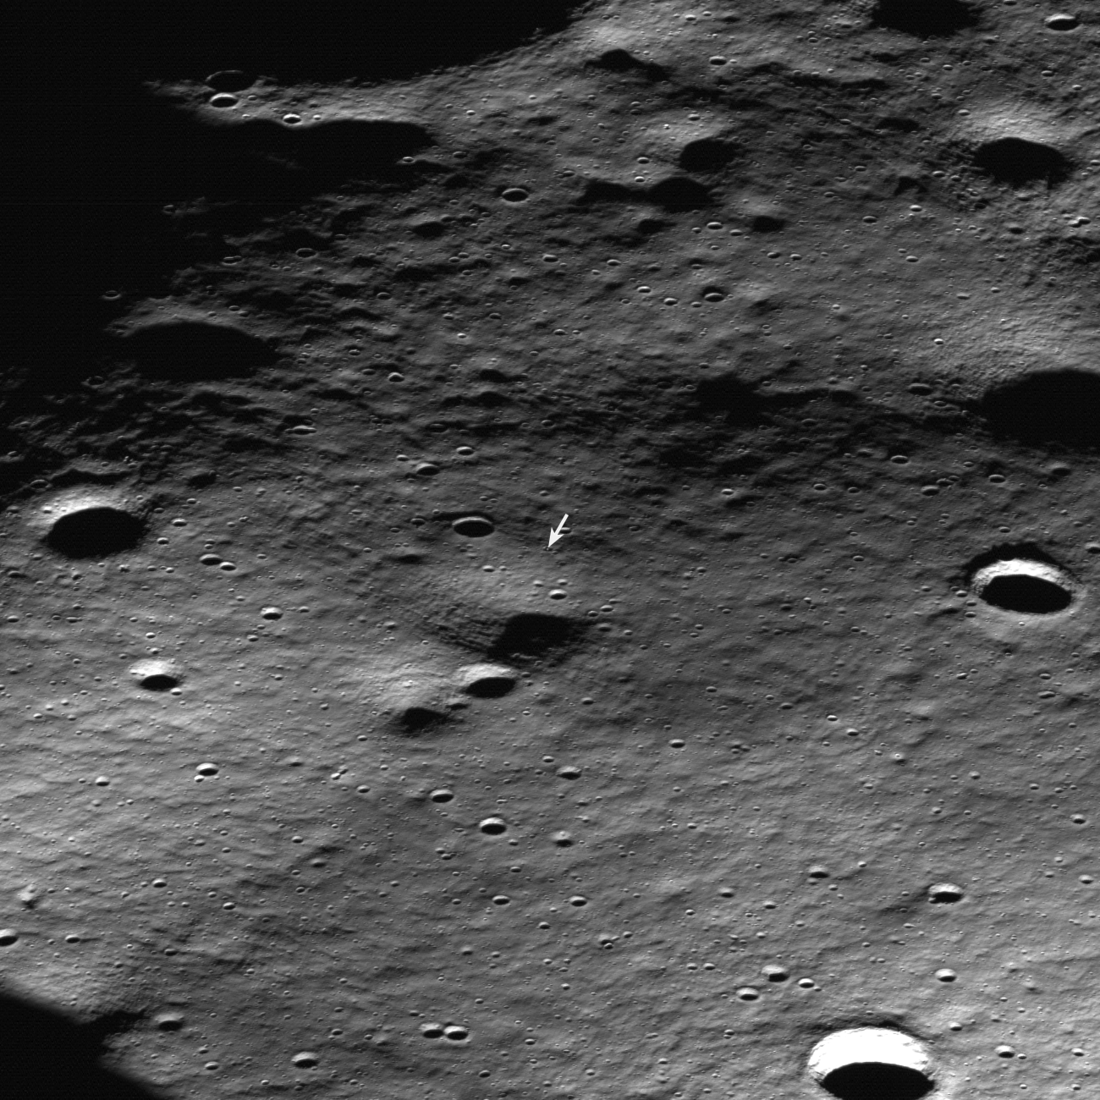
\includegraphics[width=0.82\linewidth]{athena_lroc_hero_1300p}
\caption{The IM-2 Athena landing site on Mons Mouton, lunar south pole, in an LROC
NAC oblique view acquired after the landing. The grazing polar sunlight that throws
the long shadows here is the same illumination that makes Channel~2 work. Base image:
NASA/GSFC/Arizona State University, LROC team.}
\label{fig:hero}
\end{figure}

Two rules keep the test honest. First, every input predates the landing by thirteen
years, so nothing in the pixels could have been shaped by the crash. Second, the
landing \emph{outcome} never enters the math; the only thing borrowed from after the
fact is the single coordinate telling me which pixel to read, and that pixel is
scored the same way as every other one.

\begin{intentbox}
A ``what if we had looked earlier'' study is dangerous precisely because the answer
is already known. It is easy, even unconsciously, to tune an analysis until it agrees
with reality. The two guardrails above (pre-landing-only inputs, outcome-free
scoring) are there so the result is a measurement, not a self-fulfilling prophecy.
This is a \emph{detectability} test. It is not a claim that HATI would have changed
the mission, and it is not a blind prediction, because I knew where to look.
\end{intentbox}

HATI runs two independent channels, sketched in \cref{fig:pipeline}. This paper makes
three contributions, in order. First, the \emph{architecture}: both channels are defined
from first principles --- a multi-scale roughness heatmap from the elevation model, and a
shadow census from the photograph --- together with how they fuse and why they cover
complementary size bands. Second, a \emph{forensic test}: the whole pipeline is run on
the real IM-2 Athena failure site, from pre-landing data, and the flag is decomposed
channel by channel. Third, a \emph{validation}: a resolution ladder
(\cref{sec:validation}) that hands each channel degraded data and measures how well it
recovers the hazards visible at full resolution --- the step that turns one compelling
case into a method with measured detection performance. Every block of mathematics is
followed by a plain statement of what it means, and the limitations are fenced, not
hidden. The Athena loss is the running example throughout, both because it motivates the
work and because it is the rare case with an unarguable answer key.

\begin{figure}[t]
\centering
\begin{tikzpicture}[node distance=7mm and 16mm]
  \node[io] (dtm) {NAC DTM\\\SI{4}{\meter\per\px}\\(elevation)};
  \node[io, right=of dtm] (ortho) {NAC ortho\\\SI{0.9}{\meter\per\px}\\(photograph)};
  \node[proc, below=of dtm] (feat) {Tier-1 feature stack\\(10 roughness channels)};
  \node[proc, below=of ortho] (det) {local-relative\\shadow detection};
  \node[proc, below=of feat] (fuse) {robust $z$-score\\$\to$ weighted sum\\$\to$ logistic};
  \node[proc, below=of det] (ell) {ellipse fit:\\footprint + length};
  \node[io, below=of fuse] (heat) {hazard heatmap\\$H(x)\in[0,1]$};
  \node[io, below=of ell] (cens) {sub-resolution\\obstacle census};
  \coordinate (mid) at ($(heat)!0.5!(cens)$);
  \node[dec, below=10mm of mid] (flag) {flag at\\touchdown?};
  \draw[flowarr] (dtm)--(feat); \draw[flowarr] (feat)--(fuse);
  \draw[flowarr] (fuse)--(heat); \draw[flowarr] (ortho)--(det);
  \draw[flowarr] (det)--(ell); \draw[flowarr] (ell)--(cens);
  \draw[flowarr] (heat)|-(flag); \draw[flowarr] (cens)|-(flag);
  \node[font=\footnotesize\sffamily\itshape, text width=33mm, align=left, right=8mm of flag, anchor=west]
       {success bar:\\ \emph{either} channel\\ flags the point.};
  \begin{scope}[on background layer]
    \node[draw=hatiblue!30, dashed, rounded corners, fit=(dtm)(feat)(fuse)(heat),
          inner sep=4pt, label={[hatiblue,font=\footnotesize\sffamily]above:Channel 1 \textemdash{} resolved roughness}] {};
    \node[draw=hatiteal!40, dashed, rounded corners, fit=(ortho)(det)(ell)(cens),
          inner sep=4pt, label={[hatiteal,font=\footnotesize\sffamily]above:Channel 2 \textemdash{} sub-resolution shadows}] {};
  \end{scope}
\end{tikzpicture}
\caption{The two HATI channels. Channel~1 turns the elevation model into a
ranked hazard score; Channel~2 turns the photograph into a census of obstacles too
small for the elevation model to see. The test passes if either one flags the
touchdown.}
\label{fig:pipeline}
\end{figure}

% =====================================================================
\section{Data, and the rule against cheating}

Both maps come from the LROC NAC stereo product \texttt{NAC\_DTM\_NOBILE03}
(Arizona State University; \cite{robinson2010}), built from three NAC frames acquired
on 31 August 2012:
\begin{itemize}
  \item an elevation model (DTM) at \SI{4.0}{\meter\per\px}, \num{1473}$\times$\num{1172} pixels;
  \item a co-registered orthophoto at \SI{0.9}{\meter\per\px}, \num{6547}$\times$\num{5209} pixels, 16-bit.
\end{itemize}

\begin{intentbox}
The choice of a 2012 product is the whole guardrail. Anything built from
post-landing imagery would let the crash leak into the ``prediction.'' Using source
frames from thirteen years earlier means the test is fair: the maps knew nothing
about IM-2.
\end{intentbox}

\begin{figure}[t]
\centering
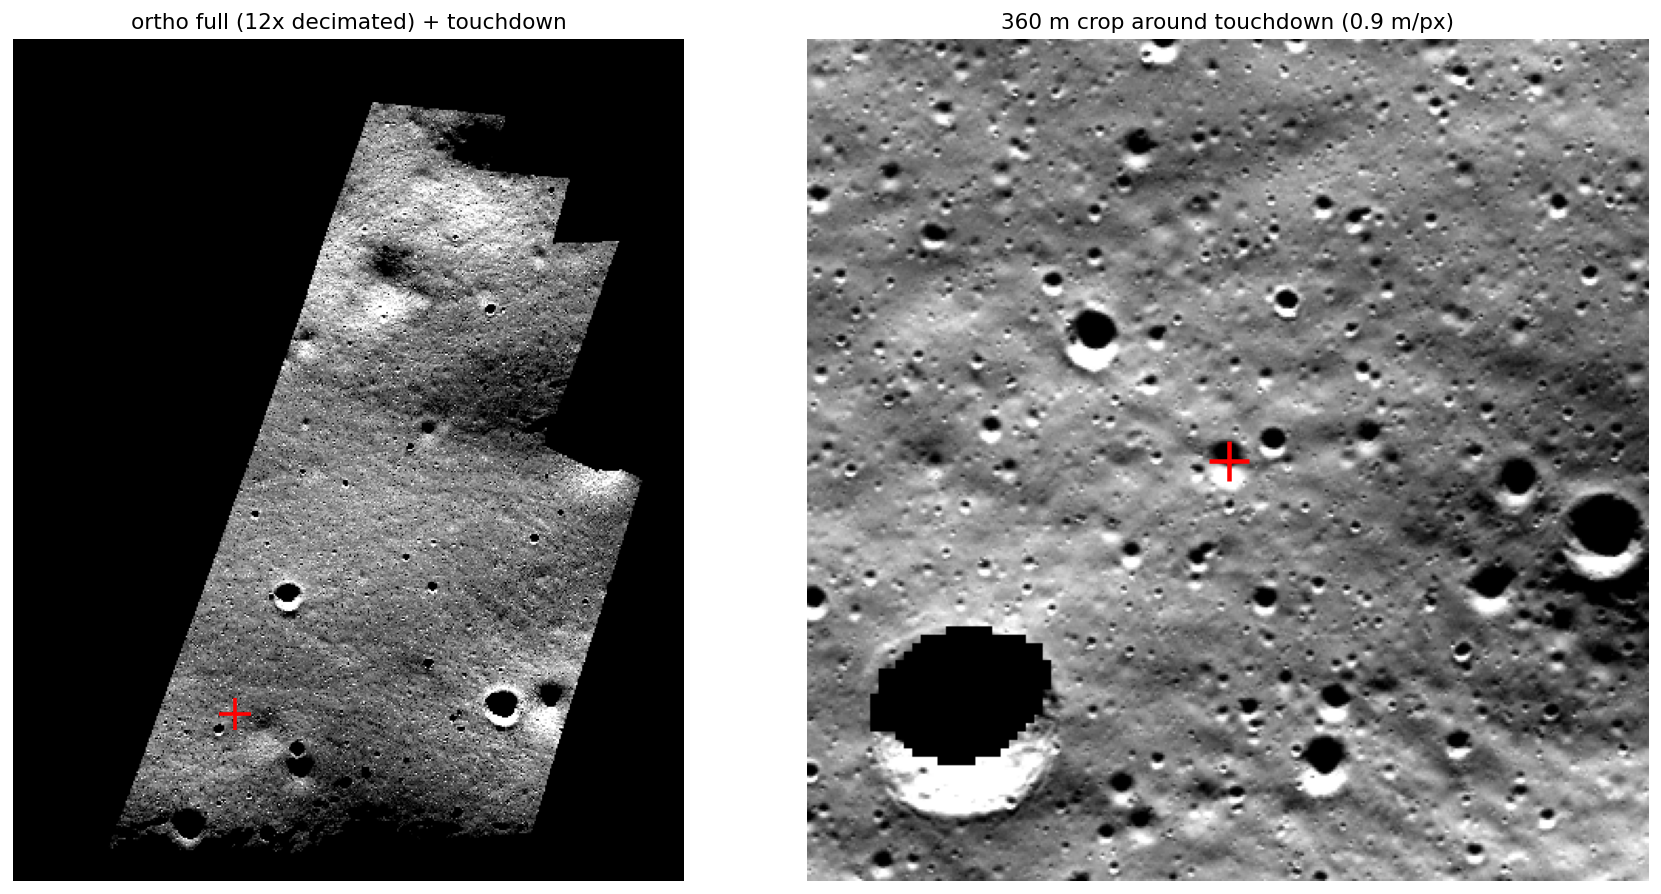
\includegraphics[width=0.92\linewidth]{ortho_probe}
\caption{Left: the full \SI{0.9}{\meter\per\px} orthophoto (the data covers a tilted
diamond inside the rectangular file; black is outside coverage), with the touchdown
marked. Right: a \SI{360}{\meter} crop around the touchdown. The point sits in a
dense field of small craters, several of which are far below the elevation model's
resolving limit. Note the pitch-black, fully shadowed interior of the large crater
at lower left: grazing polar light turns relief into long, readable shadows.}
\label{fig:ortho}
\end{figure}

% =====================================================================
\section{Finding the exact spot}

Both maps use a south-polar stereographic grid on a sphere of radius
$R=\SI{1737.4}{\kilo\meter}$, centred on the pole, longitude measured east
(\cref{fig:geo}). To convert the touchdown latitude $\varphi$ and longitude
$\lambda$ into a position on that grid I use the closed-form spherical projection,
\begin{equation}
\rho = 2R\,\tan\!\left(\frac{\pi}{4}+\frac{\varphi}{2}\right),
\qquad x = \rho\sin\lambda,\qquad y = \rho\cos\lambda ,
\label{eq:stereo}
\end{equation}
then divide by the pixel size and offset by the map corner. I ran this two
independent ways, \cref{eq:stereo} and the GDAL coordinate engine, and they land on
the same pixel with zero disagreement: row 1181, column 387 on the elevation model,
row 5248, column 1721 on the photograph.

\begin{figure}[t]
\centering
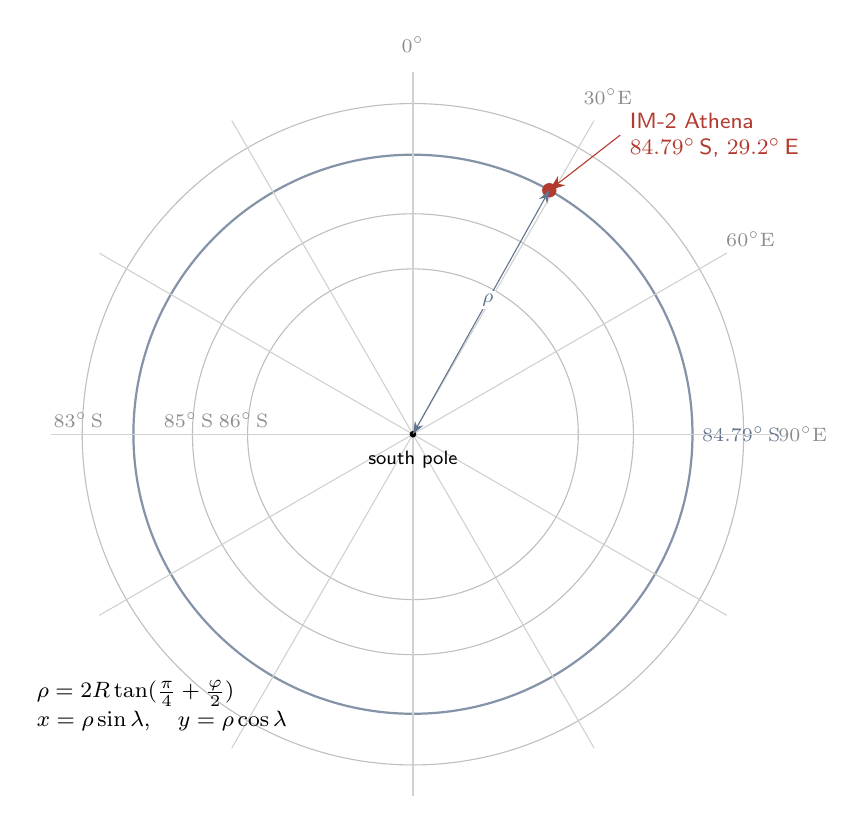
\begin{tikzpicture}[scale=1.0]
  \def\Rtd{3.55}
  % latitude circles (colatitude = 90 - |lat|)
  \foreach \r/\lab in {2.1/{\ang{86}\,S}, 2.8/{\ang{85}\,S}, 4.2/{\ang{83}\,S}} {
    \draw[black!25] (0,0) circle (\r);
    \node[black!45, font=\scriptsize] at (-\r-0.05,0.18) {\lab};
  }
  \draw[hatiblue!55, thick] (0,0) circle (\Rtd);
  \node[hatiblue!70, font=\scriptsize] at (\Rtd+0.62,0) {\ang{84.79}\,S};
  % longitude spokes
  \foreach \a in {0,30,...,330} { \draw[black!18] (0,0)--(\a+90:4.6); }
  \foreach \a/\lab in {90/{\ang{0}}, 60/{\ang{30}E}, 30/{\ang{60}E}, 0/{\ang{90}E}} {
    \node[black!45, font=\scriptsize] at (\a:4.95) {\lab};
  }
  \node[font=\scriptsize\sffamily] at (0,-0.32) {south pole};
  \fill[black] (0,0) circle (1.2pt);
  % touchdown at longitude 29.2 E -> angle from +y axis (north-up): place at (sin,cos)
  \coordinate (TD) at ({\Rtd*sin(29.2)},{\Rtd*cos(29.2)});
  \fill[hatiaccent] (TD) circle (2.6pt);
  \draw[hatiaccent, -{Stealth[length=2mm]}] (TD)++(0.9,0.7) node[right,font=\footnotesize\sffamily,align=left]
       {IM-2 Athena\\\ang{84.79}\,S, \ang{29.2}\,E} -- (TD);
  % radius annotation
  \draw[hatiblue!70, {Stealth[length=1.6mm]}-{Stealth[length=1.6mm]}] (0,0)--(TD);
  \node[hatiblue!70, font=\scriptsize, fill=white, inner sep=1pt] at ($(0,0)!0.55!(TD)$) {$\rho$};
  \node[font=\footnotesize, align=left, anchor=north west] at (-4.9,-3.0)
       {$\rho = 2R\tan(\tfrac{\pi}{4}+\tfrac{\varphi}{2})$\\[1pt]
        $x=\rho\sin\lambda,\quad y=\rho\cos\lambda$};
\end{tikzpicture}
\caption{Turning a latitude/longitude into a pixel. Looking straight down on the
south pole, lines of latitude become circles and lines of longitude become spokes. A
point's distance from the pole, $\rho$, depends only on its latitude; the spoke it
sits on is its longitude. The touchdown (red) is \ang{5.21} of latitude from the
pole, on the \ang{29.2}\,E spoke.}
\label{fig:geo}
\end{figure}

\begin{plainbox}
A stereographic map is what you get if you stand at the north pole and trace every
south-polar point onto a flat sheet. Near the pole it barely distorts anything, so
distances and shapes stay honest. Equation~\eqref{eq:stereo} is just the rule for
``how far from the centre, and in which direction'' for a given latitude and
longitude.
\end{plainbox}

% =====================================================================
\section{Channel 1: the roughness heatmap}

\subsection{The idea}
\begin{plainbox}
Picture a parking lot shot from so high up that anything smaller than a car blurs
into a smudge. You cannot see individual potholes. But a patch full of potholes still
\emph{looks} different from smooth asphalt: speckled, busy, high-variance. The
heatmap is a machine for measuring that busy-ness at several sizes at once, then
boiling it down to one hazard number between 0 and 1. A \SI{20}{\meter} crater is
only five pixels wide on a \SI{4}{\meter} map, so you will not always see the bowl,
but you will see the neighbourhood get statistically rougher. That is the signal.
\end{plainbox}

\subsection{The channels, why each one is included, and how hard each one pushed}
\label{sec:channels}

Every channel is an image the size of the elevation model, where bright means
``rough here.'' They are built from two primitives. Slope is rise over run,
\begin{equation}
s(x,y)=\arctan\sqrt{\left(\tfrac{\partial z}{\partial x}\right)^2+\left(\tfrac{\partial z}{\partial y}\right)^2},
\label{eq:slope}
\end{equation}
and curvature is the Laplacian $\nabla^2 z=\partial^2 z/\partial x^2+\partial^2 z/\partial y^2$,
positive in a bowl, negative on a dome. Each channel measures one of these inside a
small sliding window.

The cleverest family is Median Differential Slope (MDS). It blurs the terrain to two
sizes, $L$ and $2L$, measures slope on each, and subtracts. What survives is the
roughness that lives specifically around size $L$. Run it at several $L$ and you get
a little size-spectrum of bumpiness; I use $L\approx 8,12,20,32\,\si{\meter}$, which
brackets the crater Athena struck \autocite{kreslavsky2000,rosenburg2011}.

\Cref{tab:influence} is the heart of the proof of concept. It decomposes the score
\emph{at the touchdown}: each channel's $z$-score there, its literature weight, and
its additive contribution to the final logit. The contributions sum, the bias $-1.0$
is added, the logistic squashes the total, and the result is $H=0.726$. The same data
is drawn in \cref{fig:influence}.

\begin{table}[t]
\centering
\caption{Per-channel decomposition at the touchdown (config: window 7, MDS
8\textendash\SI{32}{\meter}). ``Contribution'' is each channel's additive share of
the pre-logistic score. A positive value pushes the hazard up.}
\label{tab:influence}
\small
\begin{tabular}{l S[table-format=1.2] S[table-format=-1.2] S[table-format=+1.3] S[table-format=2.1] l}
\toprule
Channel & {Weight} & {$z$ at touchdown} & {Contribution} & {Value pct.} & Push \\
\midrule
Slope IQR        & 1.00 & 4.00 & +0.476 & 98.7 & up \\
MDS @ \SI{12}{\meter} & 0.90 & 3.79 & +0.406 & 98.4 & up \\
$|$TPI$|$        & 0.70 & 4.00 & +0.333 & 99.0 & up \\
MDS @ \SI{8}{\meter}  & 1.00 & 2.69 & +0.321 & 96.0 & up \\
MDS @ \SI{20}{\meter} & 0.80 & 2.92 & +0.278 & 96.7 & up \\
Curvature IQR    & 1.00 & 1.29 & +0.153 & 85.0 & up \\
Planar deviation & 0.70 & 1.60 & +0.134 & 88.9 & up \\
MDS @ \SI{32}{\meter} & 0.60 & 0.42 & +0.030 & 64.8 & up (weak) \\
RMS slope        & 1.00 & -0.64 & -0.077 & 24.7 & \textbf{down} \\
TRI              & 0.70 & -0.94 & -0.079 & 16.2 & \textbf{down} \\
\bottomrule
\end{tabular}
\end{table}

\begin{figure}[t]
\centering
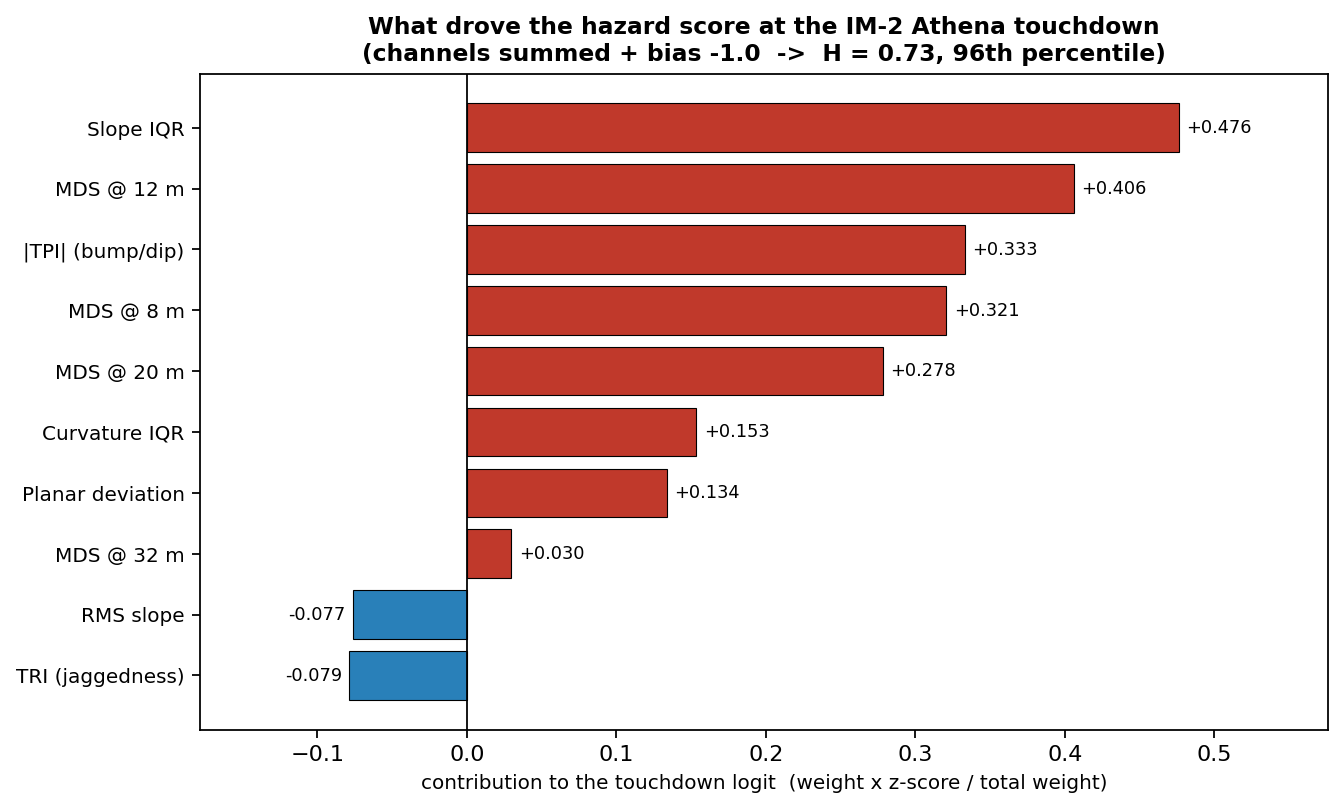
\includegraphics[width=0.86\linewidth]{athena_channel_influence}
\caption{What drove the hazard score at the touchdown. Red bars push the score up,
blue bars pull it down. The two channels that read \emph{average} tilt
(RMS slope, TRI) vote the site safe; the channels that read \emph{structured,
feature-scale} roughness overrule them.}
\label{fig:influence}
\end{figure}

\noindent Each channel, with the reason it earns a place:

\begin{description}[leftmargin=0pt,style=unboxed,itemsep=3pt]
\item[Slope IQR \textnormal{(spread of slope directions; weight 1.00; biggest driver, $+0.476$).}]
A clean plane has slopes all pointing one way, so the spread is tiny; a crater field
has slopes pointing everywhere, so the spread explodes \autocite{kreslavsky2013}. At
the touchdown it maxed out at the $+4$ clip. Fingerprint of a pitted surface.
\item[MDS @ \SI{12}{\meter} \textnormal{(roughness at the \SI{12}{\meter} size; weight 0.90; $+0.406$).}]
Differential slope isolates bumpiness at one chosen size, and \SI{12}{\meter} sits
right on the crater the LROC team blamed. This channel put its finger on the hazard's
actual size.
\item[$|$TPI$|$ \textnormal{(height above/below the local mean; weight 0.70; $+0.333$).}]
A lander cares whether it is perched on a rim or sunk in a bowl. At the 99th
percentile, the point sits on strong local relief.
\item[MDS @ \SI{8}{\meter} and @ \SI{20}{\meter} \textnormal{(weights 1.00, 0.80; $+0.321$, $+0.278$).}]
The smaller MDS sizes sit nearest the resolution floor, where an unresolved hazard
leaves its first mark, so they carry top weight \autocite{caifa2020}. Both fired
hard: the danger has structure across the whole 8\textendash\SI{20}{\meter} band.
\item[Curvature IQR and Planar deviation \textnormal{(weights 1.00, 0.70; $+0.153$, $+0.134$).}]
Craters carry a telltale curvature pattern (positive rim, negative floor); planar
deviation catches general lumpiness. Both moderately raised, backing the cratered
read without running the show.
\item[MDS @ \SI{32}{\meter} \textnormal{(weight 0.60; almost nothing, $+0.030$).}]
The coarsest size here. Its near-silence is itself a finding: the hazard is smaller
than \SI{32}{\meter}.
\item[RMS slope and TRI \textnormal{(average slope, single-step jaggedness; weights 1.00, 0.70; both \textbf{negative}).}]
And here is the line that makes the proof of concept land \autocite{rosenburg2011,riley1999}.
Both sit \emph{below} the scene median. The average tilt is gentle and the
pixel-to-pixel steps are small. On their own, these two channels call the site calm.
\end{description}

\subsubsection{The hazard signature, in one sentence}
Low average slope, low jaggedness, but maxed slope spread, near-maxed TPI, and high
MDS across 8\textendash\SI{20}{\meter}. In plain words: gently tilted and smooth
between features, yet packed with crater-scale relief. That is what a gently-sloped,
heavily-cratered patch looks like, and it is exactly the case a slope-only screen
waves through (\cref{fig:slopevtex}). The flag is not one channel shouting; it is the
disagreement between the channels that read gross tilt and the channels that read
structured roughness, settled inside a single number, from topography alone.

\begin{figure}[t]
\centering
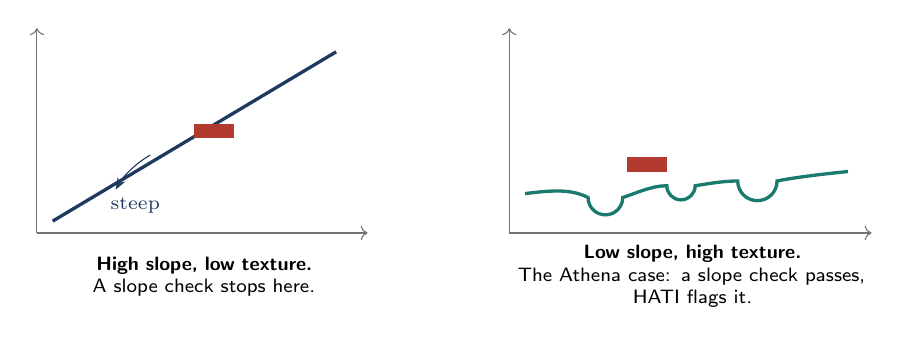
\begin{tikzpicture}[scale=1.0]
  % LEFT: steep smooth ramp
  \begin{scope}
    \draw[->,black!55] (0,0)--(4.2,0) node[right,font=\scriptsize]{};
    \draw[->,black!55] (0,0)--(0,2.6);
    \draw[very thick,hatiblue] (0.2,0.15) -- (3.8,2.3);
    \fill[hatiaccent] (2.0,1.2) rectangle ++(0.5,0.18); % lander
    \node[font=\scriptsize\sffamily,align=center,text width=42mm] at (2.1,-0.55)
      {\textbf{High slope, low texture.}\\ A slope check stops here.};
    \draw[hatiblue,{Stealth[length=1.5mm]}-] (1.0,0.55) arc (150:120:1.2);
    \node[hatiblue,font=\scriptsize] at (1.25,0.35) {steep};
  \end{scope}
  % RIGHT: gentle cratered surface
  \begin{scope}[xshift=6.0cm]
    \draw[->,black!55] (0,0)--(4.6,0);
    \draw[->,black!55] (0,0)--(0,2.6);
    % gentle baseline with crater dips
    \draw[very thick,hatiteal]
      (0.2,0.5)
      .. controls (0.6,0.55) and (0.8,0.55) .. (1.0,0.45)
      arc (180:360:0.22)
      .. controls (1.6,0.5) and (1.8,0.6) .. (2.0,0.6)
      arc (180:360:0.18)
      .. controls (2.5,0.62) and (2.7,0.66) .. (2.9,0.66)
      arc (180:360:0.25)
      .. controls (3.6,0.7) and (3.9,0.74) .. (4.3,0.78);
    \fill[hatiaccent] (1.5,0.78) rectangle ++(0.5,0.18);
    \node[font=\scriptsize\sffamily,align=center,text width=46mm] at (2.3,-0.55)
      {\textbf{Low slope, high texture.}\\ The Athena case: a slope check passes,\\ HATI flags it.};
  \end{scope}
\end{tikzpicture}
\caption{Why ``low slope'' is not ``safe.'' A steep clean ramp (left) is caught by an
ordinary slope check. A gently-tilted but crater-pocked surface (right) passes that
check while being genuinely dangerous. Channel~1 is built to separate these two.}
\label{fig:slopevtex}
\end{figure}

\subsection{Filling the holes in the map}
The elevation file is a rectangle, but the real data fills only a tilted diamond
inside it; about \SI{45}{\percent} is ``no data.'' Sliding-window math across the
cliff between real data and a hole produces garbage spikes.

\begin{intentbox}
I fill every hole with the value of its \emph{nearest real pixel} before any window
math, so the filled region is a smooth continuation instead of a cliff. Then, after
computing the channels, I discard every pixel close enough to a hole that a window
could have peeked in. The touchdown sits \SI{116}{\meter} from the nearest hole, far
enough that the 8\textendash\SI{32}{\meter} channels never reach the edge.
\end{intentbox}

\subsection{Folding ten channels into one number}
Each channel is first normalised by a robust $z$-score, using the median and the
inter-quartile range (IQR) rather than the mean and standard deviation, after a
$\log(1+\cdot)$ squash and a clip at $\pm 4$:
\begin{equation}
z_k=\operatorname{clip}_{\pm4}\!\left(\frac{g(c_k)-\operatorname{med}\,g(c_k)}{\operatorname{IQR}g(c_k)/1.349}\right),\qquad g(\cdot)=\log(1+\cdot).
\label{eq:z}
\end{equation}
Then a literature-weighted sum, normalised by the total weight, shifted by a bias,
and squashed to $[0,1]$ by the logistic $\sigma$:
\begin{equation}
H=\sigma\!\left(\frac{\sum_k w_k z_k}{\sum_k |w_k|}+b\right),\qquad
\sigma(t)=\frac{1}{1+e^{-t}},\qquad b=-1.0 .
\label{eq:fuse}
\end{equation}

\begin{intentbox}
Three deliberate choices. The median/IQR (not mean/standard-deviation) means a few
freak pixels cannot hijack the scale. The $\log(1+\cdot)$ tames the long tail of
roughness so flat terrain still spreads out usefully. Dividing by the total weight
decouples the score from the number of channels, so adding or removing one does not
silently move the midpoint. The weights come from the roughness literature, not from
tuning against Athena.
\end{intentbox}

\begin{limitbox}
$H$ is a \emph{relative} score: it ranks each pixel against the rest of this scene.
``96th percentile'' means rougher than \SI{96}{\percent} of the Mons Mouton massif,
and that massif is rough everywhere. Turning a ranking into an absolute hazard needs
a calibration baseline; see \cref{sec:future}.
\end{limitbox}

\subsection{Reading the score, without fishing for it}
The honest worry with any multi-knob method is that the knobs were turned until the
site looked guilty. To kill that worry I swept window sizes and MDS bands and report
\emph{all} of them, including the one that fails (\cref{tab:sweep}).

\begin{table}[t]
\centering
\caption{Robustness sweep. Every configuration that can be \emph{computed} at this
near-edge site puts the touchdown in the worst 4\textendash\SI{7}{\percent}. The
Apollo-default config returns ``undefined'' because its \SI{80}{\meter} scale reaches
the data edge \SI{116}{\meter} away.}
\label{tab:sweep}
\small
\begin{tabular}{l l c c c}
\toprule
Configuration & MDS sizes & $H$ at touchdown & Scene percentile & Flag ($>$p75 / p90) \\
\midrule
Apollo default (win.\ 11) & 12\textendash\SI{80}{\meter} & {undefined} & {\textemdash} & {\textemdash} \\
window 5 & 8\textendash\SI{32}{\meter} & 0.757 & 97.1 & yes / yes \\
window 7 & 8\textendash\SI{32}{\meter} & 0.726 & 96.3 & yes / yes \\
window 9 & 8\textendash\SI{24}{\meter} & 0.645 & 93.3 & yes / yes \\
window 7 & 8\textendash\SI{20}{\meter} & 0.780 & 97.4 & yes / yes \\
\bottomrule
\end{tabular}
\end{table}

At the touchdown the score is $H=0.726$, the 96.3rd percentile; only
\SI{3.7}{\percent} of the valid terrain scores rougher, which is \num{3.22} robust
standard deviations above the median. Meanwhile the slope there is \ang{2.8} against
a scene median of \ang{5.1}: the point is in the \emph{15.9th} percentile for slope,
smoother than \SI{84}{\percent} of the area. Smoother than most of the site by tilt,
rougher than almost all of it by texture.

\subsection{Safe-ground control: which channels truly discriminate}
\label{sec:control}

A flag means something only if the same channels stay quiet over safe ground. To test
that without leaving the scene, I contrast the touchdown against the smoothest patch in
the \emph{same} NOBILE03 model, \SI{0.62}{\kilo\meter} away: there $H=0.072$ and the
slope is \ang{0.9}, against the touchdown's $H=0.726$ and \ang{2.8}. Product,
resolution and scene normalisation are all held fixed, so the only thing that changes
between the two points is the terrain, and their $z$-scores are directly comparable.

\begin{intentbox}
Why not run the pipeline on a separate mare scene, the obvious ``safe control''? Two
traps. Roughness is scale-dependent, so a control model at a different pixel size (the
\SI{1.5}{\meter\per\px} Apollo 17 model on disk, say) would compare different physical
scales. And the $z$-score is normalised per scene, so scores from two separate runs are
not on the same ruler. Holding scene, product and resolution fixed removes both. An
external mare control is still worth doing, but only if it matches resolution and
compares raw (or commonly-normalised) values, not per-scene $z$.
\end{intentbox}

\begin{figure}[t]
\centering
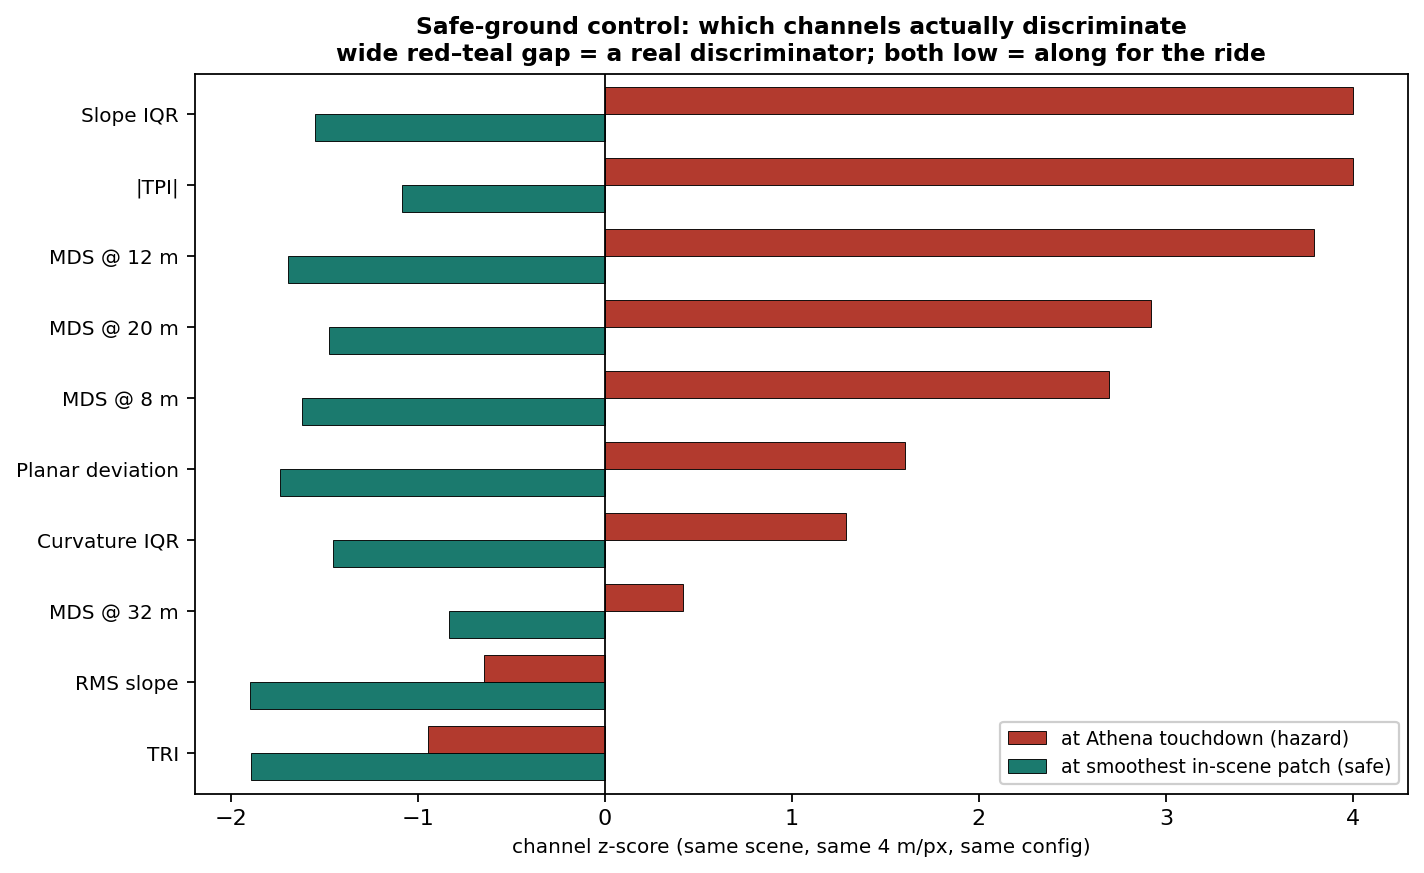
\includegraphics[width=0.84\linewidth]{athena_safe_control}
\caption{The safe-ground control. For each channel, the $z$-score at the touchdown
(red) and at the smoothest in-scene patch (teal). A wide gap means the channel
separates hazard from safe ground; two low bars mean it does not. Slope IQR, the MDS
8\textendash\SI{20}{\meter} family and $|$TPI$|$ carry the discrimination; RMS slope
and TRI barely move.}
\label{fig:control}
\end{figure}

This is the ``trained eye.'' Ranked by discrimination $z_\text{hazard}-z_\text{safe}$,
the leaders are Slope IQR ($+5.6$), MDS @ \SI{12}{\meter} ($+5.5$), $|$TPI$|$ ($+5.1$),
and MDS @ \SI{20}{\meter} and \SI{8}{\meter} ($+4.4$, $+4.3$). At the bottom sit RMS
slope ($+1.3$) and TRI ($+0.9$), both \emph{below} the scene median at the hazard
\emph{and} at safe ground. The channels that do the real work read variability and
feature-scale structure; the gross-tilt channels are along for the ride. That is the
empirical signature separating safe terrain from unsafe, and it is what a single
positive site can legitimately deliver: not just ``HATI flagged Athena,'' but which
measurements made it flag.

\begin{limitbox}
The in-scene reference is the smoothest \emph{highland} patch, not a mare, so this
shows which channels discriminate \emph{within} this terrain, not the absolute
safe-ground floor. It is also picked as the lowest-$H$ patch, so the discrimination
ranking is partly self-consistent by construction; an independently chosen flat
reference, or the external resolution-matched mare control (\cref{sec:future}), would
remove that coupling. The ranking should hold regardless, because RMS slope and TRI
sit low at the hazard \emph{too} ($z<0$), which the choice of a low-$H$ reference does
not force.
\end{limitbox}

% =====================================================================
\section{Channel 2: the shadow census}

\subsection{The idea, and the geometry of a shadow}
\begin{plainbox}
The elevation model stops at \SI{4}{\meter}. The photograph is finer than
\SI{1}{\meter}, and at the south pole the sun barely clears the horizon, so even a
knee-high rock throws a long shadow. Those shadows are free measurements of objects
far too small to appear on the elevation model.
\end{plainbox}

A shadow gives two separate numbers (\cref{fig:shadowgeo}). Its width \emph{across}
the sun is the object's true footprint, independent of how low the sun is. Its length
\emph{along} the sun gives the object's height through
\begin{equation}
h = L\,\tan e,
\label{eq:relief}
\end{equation}
where $e$ is the solar elevation. For this paper the footprint is the headline,
because it needs no assumption about the sun angle.

\begin{figure}[t]
\centering
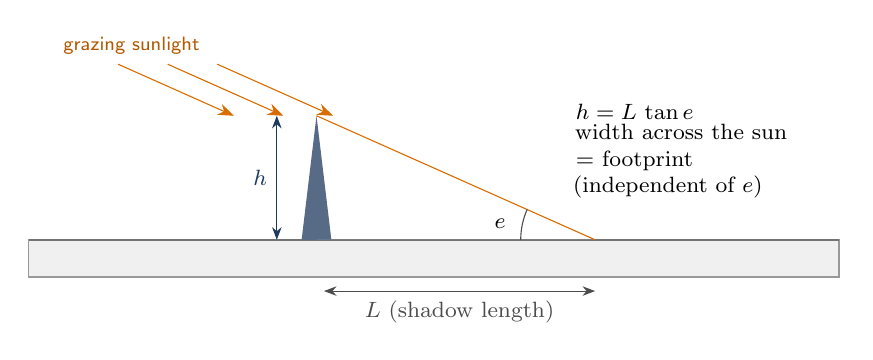
\begin{tikzpicture}[scale=1.05]
  \def\e{24} % sun elevation
  \draw[fill=black!6,draw=black!40] (-0.3,0) rectangle (9.5,-0.45); % ground
  \draw[thick,black!55] (-0.3,0)--(9.5,0);
  % obstacle
  \def\hh{1.5}
  \fill[hatiblue!75] (3,0) -- (3.18,\hh) -- (3.36,0) -- cycle;
  \coordinate (T) at (3.18,\hh);
  % shadow tip: L = h/tan e from base
  \pgfmathsetmacro{\LL}{\hh/tan(\e)}
  \coordinate (S) at ({3.18+\LL},0);
  \fill[black!22] (3.18,0) -- (S) -- (3.36,0) -- cycle;
  % sun rays parallel to T->S
  \foreach \dx in {-1.0,-0.4,0.2} {
    \draw[-{Stealth[length=2mm]},orange!85!black]
      ($(T)+(\dx,0)+(-1.4,{1.4*tan(\e)})$) -- ($(T)+(\dx,0)$);
  }
  \draw[orange!85!black] (T) -- (S);
  % angle e at S
  \draw[black!70] (S)++(-0.9,0) arc (180:{180-\e}:0.9);
  \node[font=\footnotesize] at ($(S)+(-1.15,0.2)$) {$e$};
  % height h
  \draw[{Stealth[length=1.6mm]}-{Stealth[length=1.6mm]},hatiblue] (2.7,0)--(2.7,\hh)
       node[midway,left,font=\footnotesize]{$h$};
  % length L
  \draw[{Stealth[length=1.6mm]}-{Stealth[length=1.6mm]},black!70] (3.27,-0.62)--($(S)+(0,-0.62)$)
       node[midway,below,font=\footnotesize]{$L$ (shadow length)};
  % relief formula
  \node[font=\footnotesize, anchor=west] at (6.2,1.55) {$h = L\,\tan e$};
  \node[font=\footnotesize, anchor=west, text width=33mm] at (6.2,0.95)
       {width across the sun\\ $=$ footprint\\ (independent of $e$)};
  \node[font=\scriptsize\sffamily,orange!70!black,anchor=west] at (0.0,2.35) {grazing sunlight};
\end{tikzpicture}
\caption{Shadow geometry. The cast shadow's length $L$ converts to the object's
height through the solar elevation $e$ (Eq.~\ref{eq:relief}); the width across the sun
direction is the object's footprint and does not depend on $e$. Lower sun means longer
shadows, so smaller objects become visible, which is why the south pole is the best
place for this method.}
\label{fig:shadowgeo}
\end{figure}

\subsection{Why the obvious method fails at the pole}
The naive detector calls any dark pixel a shadow. At the pole that fails badly,
because half the darkness is not cast shadow at all, it is slopes tilted away from
the grazing sun. A global brightness threshold (Otsu) labels \SI{54}{\percent} of the
crop ``shadow,'' which is meaningless.

\begin{intentbox}
The fix is to define a shadow \emph{relative to its surroundings}. I build a local
brightness baseline with a \SI{40}{\meter} median filter, then call a pixel a shadow
only if it is darker than half that local baseline. This adapts to the overall light
gradient and isolates genuine cast shadows; the dark fraction drops to a sensible
\SI{5}{\percent} and, as \cref{fig:shadow} shows, it lights up crater interiors rather
than gentle slopes.
\end{intentbox}

\subsection{From dark blobs to measured obstacles, and the resolution floor}
After thresholding I clean the mask (one morphological opening to kill speckle, one
closing to seal pinholes), label the connected blobs, and fit an ellipse to each one
of at least 4 pixels. The short axis is the cross-sun footprint, the long axis is the
shadow length. By the sampling theorem \autocite{shannon1949}, the \SI{4}{\meter}
elevation model cannot register anything below $2\times\SI{4}{\meter}=\SI{8}{\meter}$,
so I split every obstacle at that floor.

\begin{figure}[t]
\centering
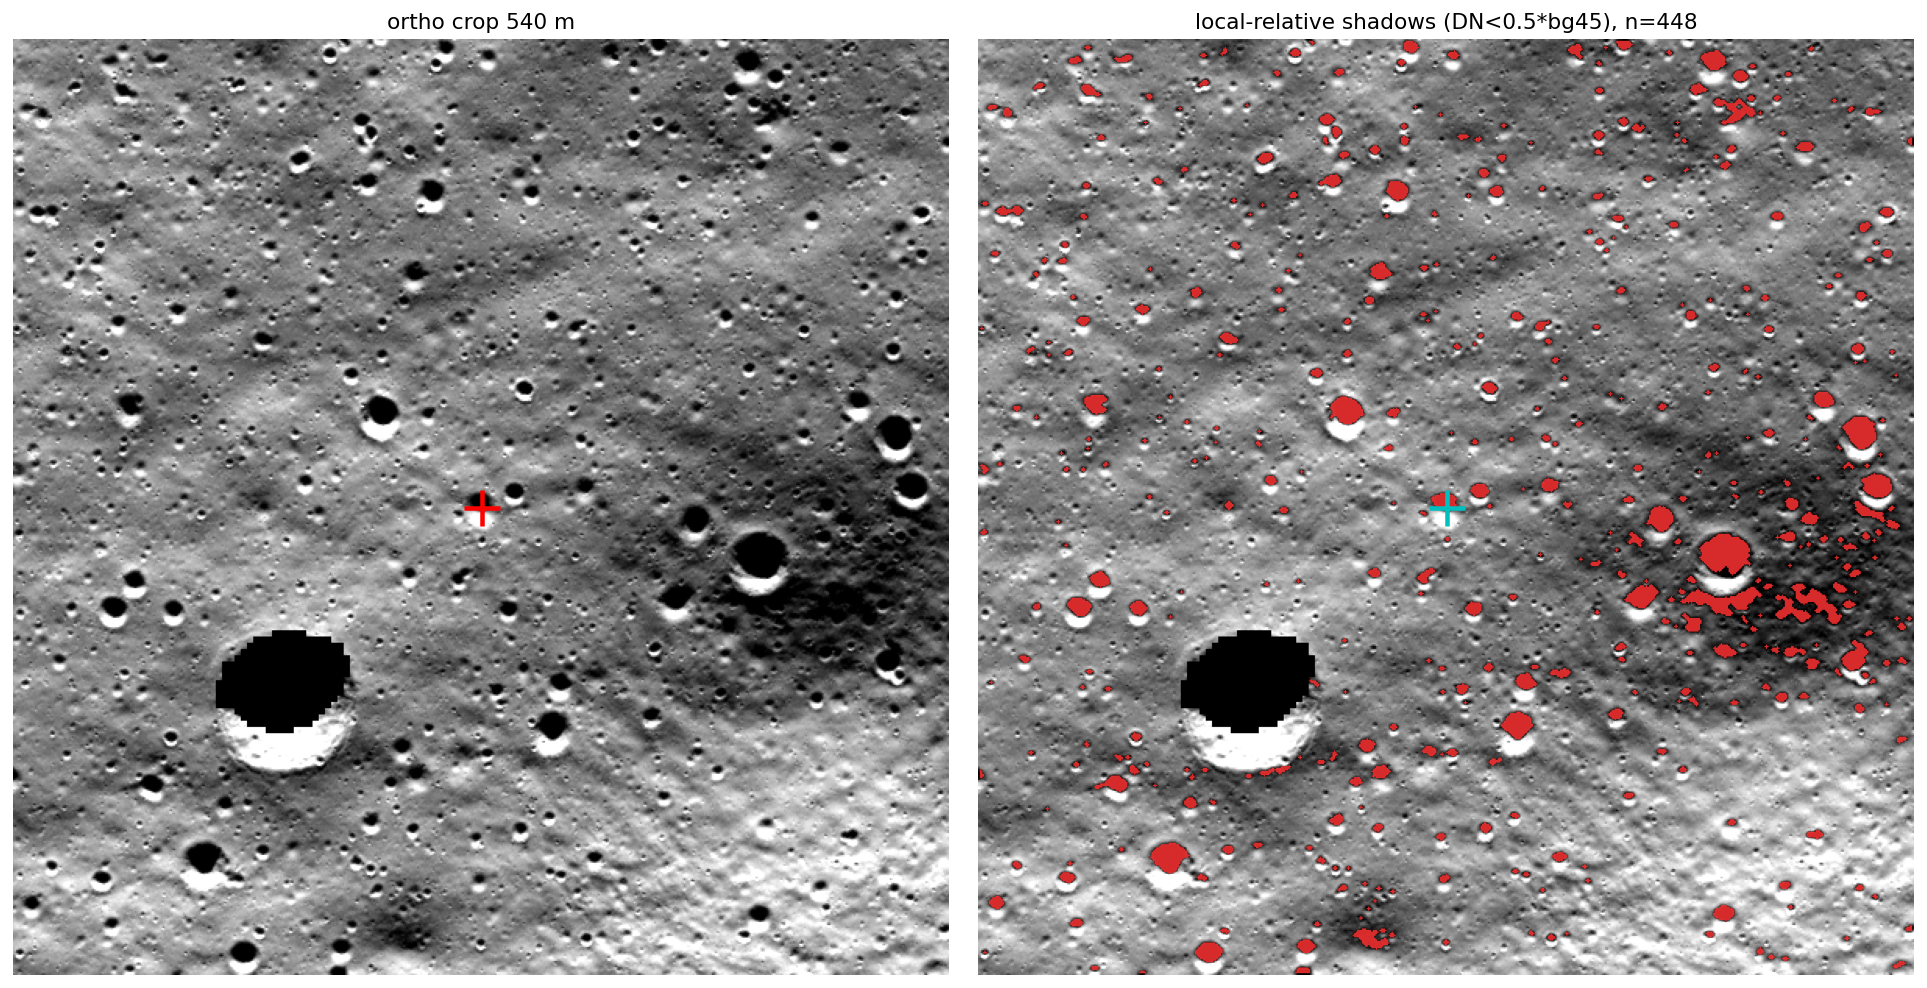
\includegraphics[width=0.92\linewidth]{shadow_probe}
\caption{Left: the orthophoto crop. Right: detected cast shadows (red) from the
local-relative method. The detector picks out the large crater's shadowed interior
and the small craters throughout, while ignoring the broad slope shading. The
touchdown (cyan) sits in the obstacle field.}
\label{fig:shadow}
\end{figure}

\subsection{A built-in lie detector, and the census}
If these ``shadows'' were random noise their orientations would point everywhere.
Real cast shadows all lean away from the sun, so they should share one direction. The
measured dominant orientation is \ang{85}, sharply single-peaked: the signature of
illumination-driven shadows, not albedo splotches.

Over a \SI{1.08}{\kilo\meter\squared} box around the touchdown the census finds
\num{1639} shadows ($\sim$\num{1514} per \si{\kilo\meter\squared}), of which
\SI{93.6}{\percent} have footprints below the \SI{8}{\meter} floor, roughly
\num{1417} per \si{\kilo\meter\squared} of obstacles the elevation model cannot
resolve, with a median footprint of \SI{3.2}{\meter}. Within \SI{25}{\meter} of the
touchdown there are 3 such sub-resolution obstacles, 9 within \SI{50}{\meter}.

\begin{limitbox}
The touchdown is \emph{not} a local density spike: its obstacle density is the median
for this region. The reason is almost worse than a spike: the whole site is uniformly
carpeted with sub-resolution obstacles, so there was no quiet pocket to retarget into.
Channel~2 therefore does not independently single out the pixel. It measures a thick
hazard layer the elevation model never showed anyone. The shadow count also scales
with the threshold ($\sim$twofold), so densities are an order of magnitude,
$\sim 10^{3}\,\si{\per\kilo\meter\squared}$, not a precise figure.
\end{limitbox}

% =====================================================================
\section{Both channels together}

\Cref{fig:money} puts the whole test on one page. Channel~1 ranks the exact touchdown
in the worst \SI{4}{\percent} of the area, on texture rather than tilt. Channel~2
shows the same area saturated with obstacles below the planning resolution. One
pinpoints the spot; both agree the site was dangerous at the scale the mission could
see and at the scale it could not.

\begin{figure}[t]
\centering
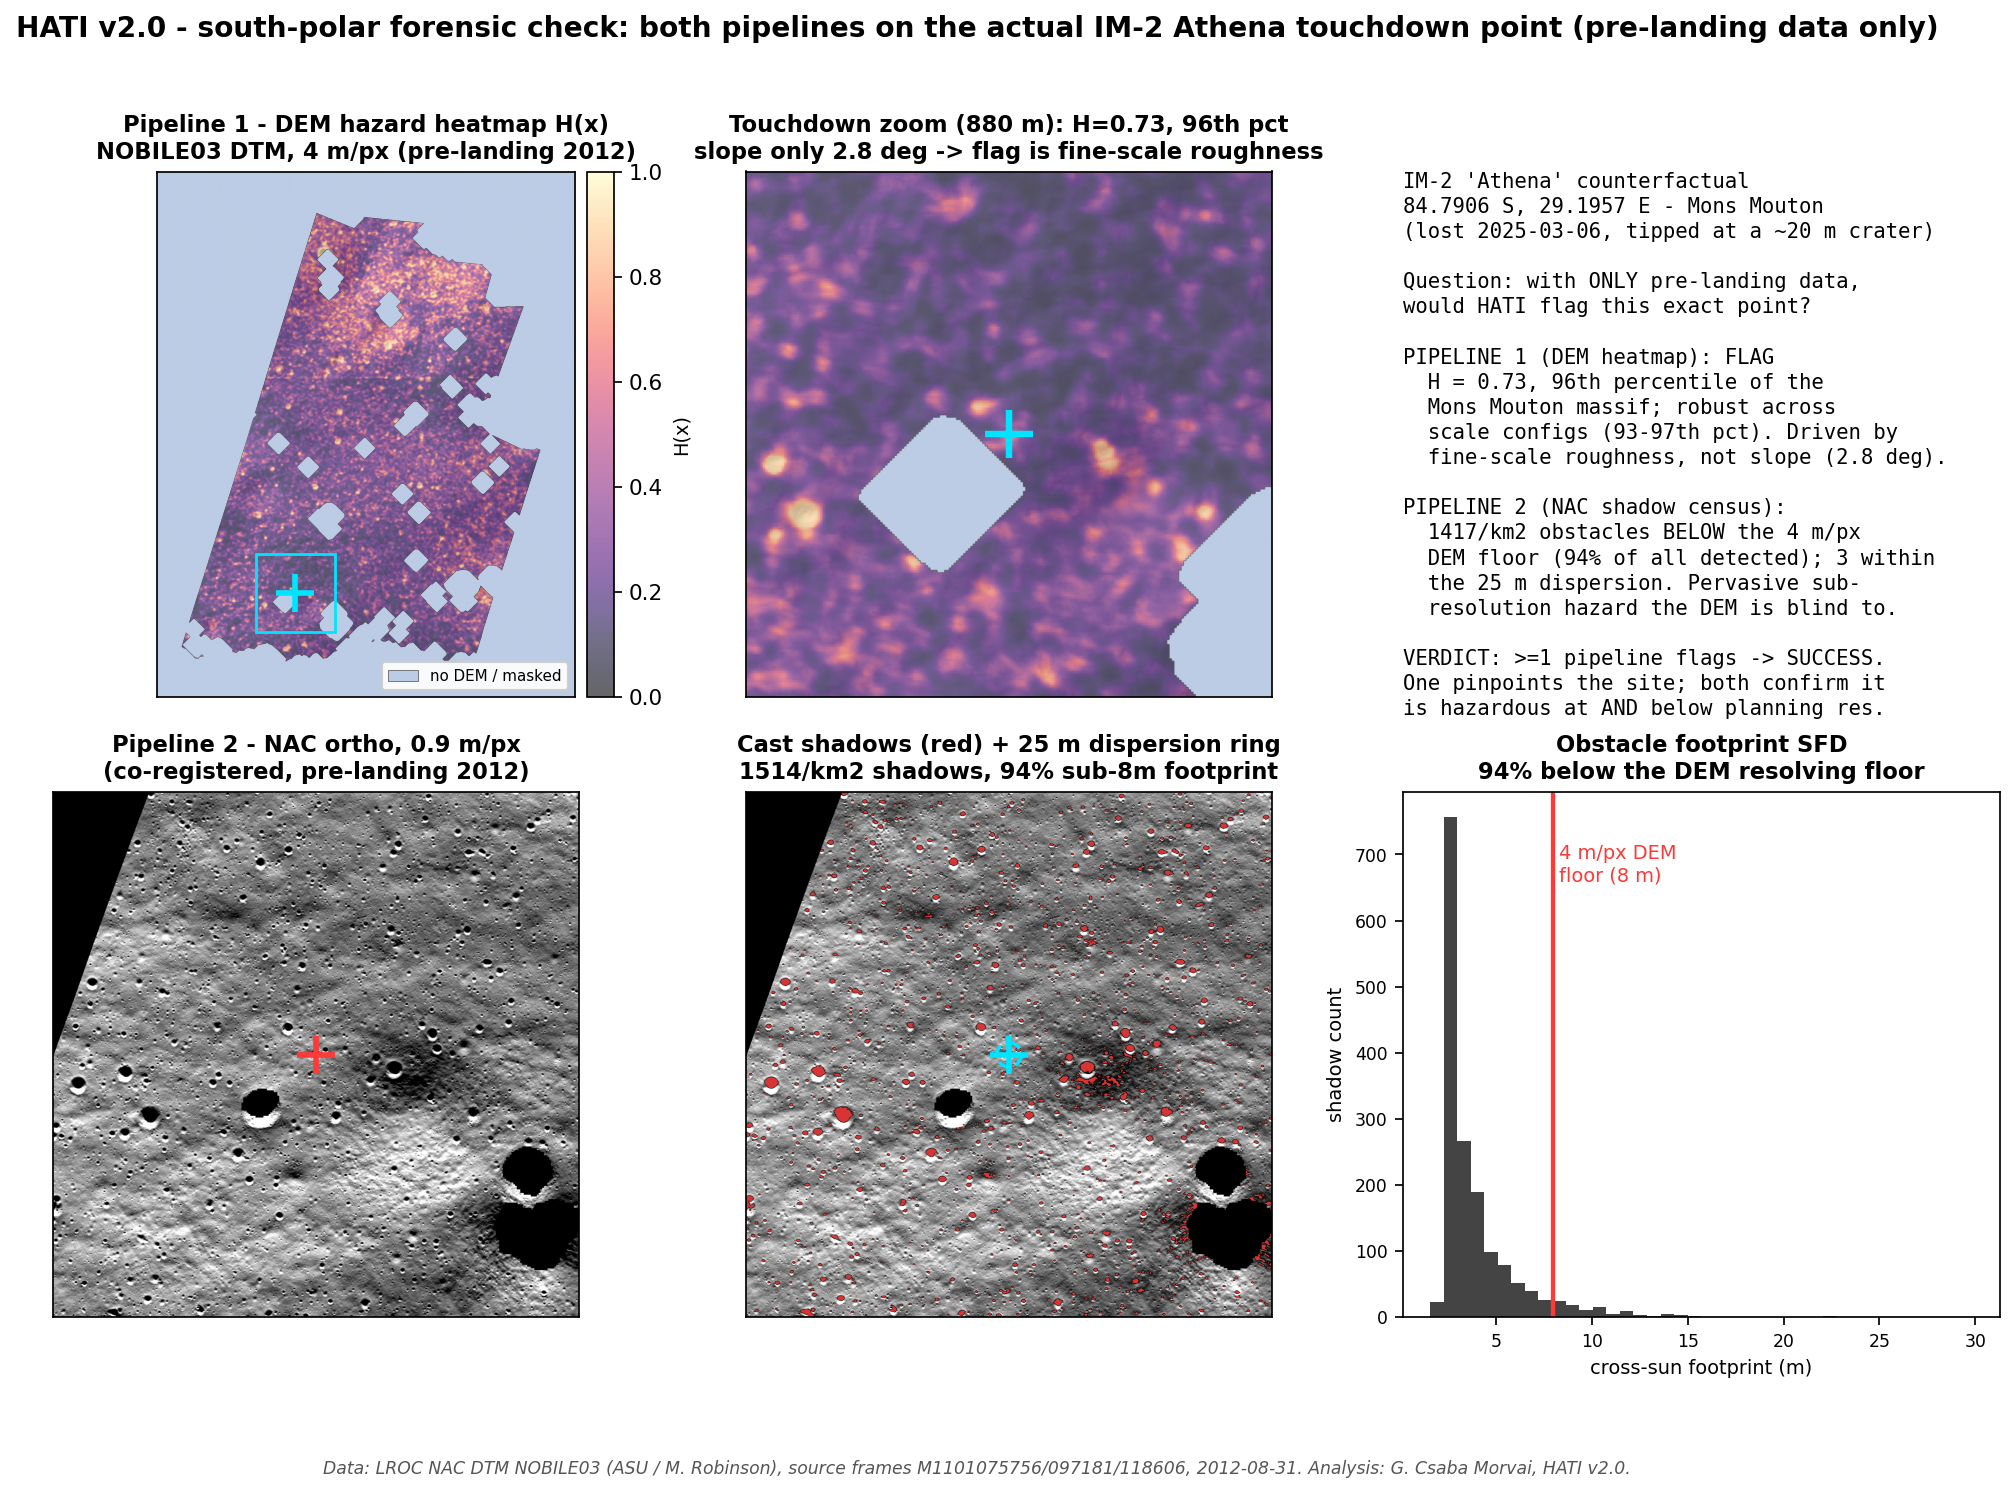
\includegraphics[width=\linewidth]{athena_counterfactual}
\caption{The full counterfactual. Top row, Channel~1: the hazard heatmap over the
massif, a zoom on the touchdown ($H=0.73$, 96th percentile, slope only \ang{2.8}),
and the verdict. Bottom row, Channel~2: the orthophoto, the detected shadows with the
\SI{25}{\meter} dispersion ring, and the obstacle footprint distribution with
\SI{94}{\percent} below the \SI{8}{\meter} floor. Light-slate areas in the top row are
no-DEM/masked regions, not terrain.}
\label{fig:money}
\end{figure}

The success bar was: if either channel flags the point, the test passes. Channel~1
flags it. The test passes. I do not upgrade this to ``both channels flag it,'' because
Channel~2's density at the point is median, and saying otherwise would be dishonest.

% =====================================================================
\section{The channel we did not build: Hapke photometric roughness ($\bar\theta$)}

HATI has no photometric-roughness channel. The Hapke scattering model carries a
parameter $\bar\theta$ (``theta-bar,'' an \emph{angle}, the mean photometric slope),
which measures roughness \emph{below} the size of a single pixel by reading how
sunlight scatters across different sun-and-camera angles \autocite{hapke1984}. The
state of the art for the Moon is the near-global $\bar\theta$ map of
\textcite{sato2014}, built from LROC Wide Angle Camera photometry, but binned at
$1^\circ\times1^\circ$ tiles, roughly \SI{30}{\kilo\meter} on a side. HATI does not
compute $\bar\theta$ at all, and yet the hazard still shows up through two channels of
pure geometry.

\begin{figure}[t]
\centering
\resizebox{\linewidth}{!}{%
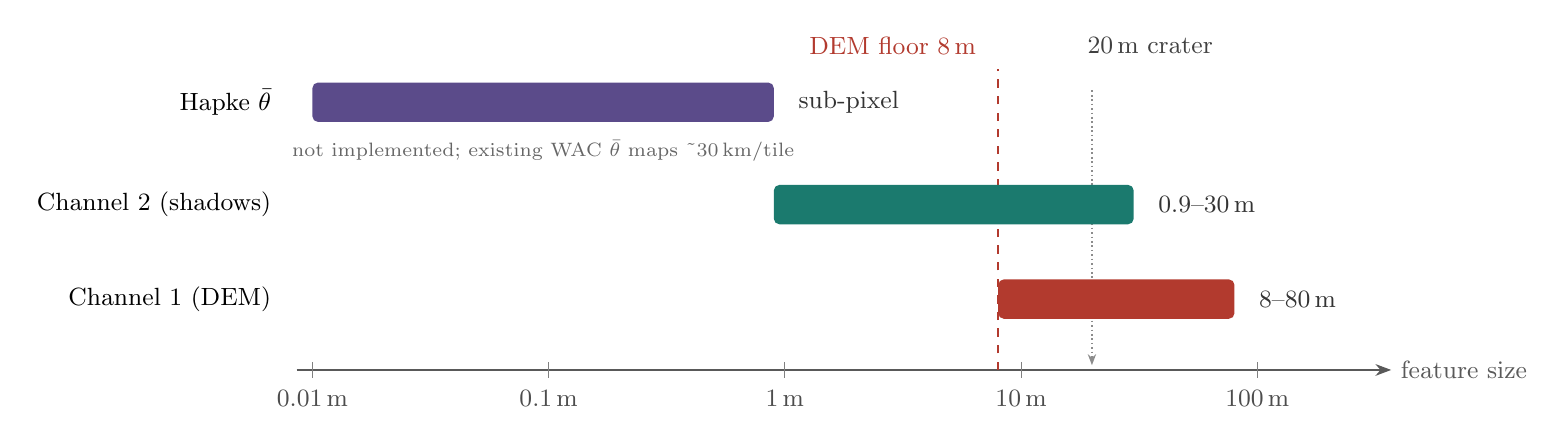
\begin{tikzpicture}[font=\sffamily]
  % log feature-size axis: x = (log10(size)+2)*3 -> 0.01,0.1,1,10,100 at 0,3,6,9,12
  \draw[-{Stealth[length=2mm]},black!65] (-0.2,0)--(13.7,0);
  \node[anchor=west,font=\small,black!65] at (13.7,0) {feature size};
  \foreach \x/\lab in {0/{0.01},3/{0.1},6/{1},9/{10},12/{100}}{
    \draw[black!50] (\x,0.1)--(\x,-0.1);
    \node[below=1pt,font=\small,black!70] at (\x,-0.1) {\lab\,m};
  }
  % markers: DEM floor (red dashed) and 20 m crater (gray dotted, points to axis)
  \draw[dashed,hatiaccent,thick] (8.71,0)--(8.71,3.82);
  \draw[densely dotted,black!45,semithick,-{Stealth[length=1.4mm]}] (9.9,3.55)--(9.9,0.06);
  \node[anchor=east,font=\small,hatiaccent] at (8.55,4.12) {DEM floor 8\,m};
  \node[anchor=west,font=\small,black!75] at (9.72,4.12) {20\,m crater};
  % band-name column (left)
  \node[anchor=east,font=\small] at (-0.4,3.40) {Hapke $\bar\theta$};
  \node[anchor=east,font=\small] at (-0.4,2.10) {Channel 2 (shadows)};
  \node[anchor=east,font=\small] at (-0.4,0.90) {Channel 1 (DEM)};
  % bands
  \fill[hatipurple,rounded corners=2pt] (0,3.15) rectangle (5.86,3.65);
  \fill[hatiteal,rounded corners=2pt]   (5.86,1.85) rectangle (10.43,2.35);
  \fill[hatiaccent,rounded corners=2pt] (8.71,0.65) rectangle (11.71,1.15);
  % right range labels (kept clear of the two markers)
  \node[anchor=west,font=\small,black!80] at (6.05,3.40) {sub-pixel};
  \node[anchor=west,font=\small,black!80] at (10.62,2.10) {0.9\textendash30\,m};
  \node[anchor=west,font=\small,black!80] at (11.90,0.90) {8\textendash80\,m};
  % Hapke caveat, on its own line under the bar, clear of bands and markers
  \node[anchor=north,font=\scriptsize,black!60,align=center] at (2.93,3.04)
       {not implemented; existing WAC $\bar\theta$ maps \textasciitilde30\,km/tile};
\end{tikzpicture}%
}
\caption{The three roughness measurements sit in different size bands. Channels 1 and
2 cover 8\textendash\SI{80}{\meter} and 0.9\textendash$\sim$\SI{30}{\meter}.
Hapke $\bar\theta$ covers the sub-pixel band neither touches, and the only existing
lunar $\bar\theta$ maps are spatially coarse ($\sim$\SI{30}{\kilo\meter} tiles). So a
$\bar\theta$ channel is not redundant with HATI; it would add an independent, finer
measurement.}
\label{fig:bands}
\end{figure}

\begin{plainbox}
The thing to be proud of, stated precisely: the hazard signal does not depend on the
hard, model-heavy machinery. It falls out of first-principles geometry, through two
independent routes that agree. When a result survives that kind of triangulation you
trust it more, because two unrelated physical mechanisms would have to fail the same
way to fool you.
\end{plainbox}

\begin{limitbox}
Two things not to oversell. First, $\bar\theta$ is \emph{not} redundant with what was
built: it reads a sub-pixel band (\cref{fig:bands}) that neither channel touches, and
you cannot even fit it from the single frame used here, because the inversion needs
multi-angle photometry. ``Not implemented'' is partly ``not implementable from this
data,'' which makes the geometric result more impressive, not less. Second, calling
the result a ``characteristic signal \emph{of hazards}'' is a specificity claim:
shown at one hazard, not yet shown to stay quiet over safe ground. Until the control
of \cref{sec:future} runs, the honest phrasing is ``a strong, two-channel signal at a
known hazard.''
\end{limitbox}

% =====================================================================
\section{Validation: a resolution ladder}
\label{sec:validation}

The forensic test is one site scored against itself; it does not, on its own, say how
well the pipelines \emph{detect}. A resolution ladder answers that with a single
controlled variable. Take data in which the hazards are directly visible, blur it to a
coarser resolution by area-averaging (the way a real coarser sensor integrates light;
naive subsampling would alias and manufacture fake roughness), run the pipeline on the
coarse version, and score it against the full-resolution detections as ground truth.
Only the resolution changes, so the result is about resolution alone.

\subsection{The shadow channel: a measured reach}
Degrading the \SI{0.9}{\meter\per\px} ortho in steps and re-running the detector at each,
the per-pixel detection performance (area under the ROC, \cref{fig:valcurves} left) holds
up as the data worsens: AUC $0.99$, $0.97$, $0.94$, $0.88$, $0.83$ at $1.8$, $2.7$, $3.6$,
$5.4$, \SI{7.2}{m}. Stratifying recovery by obstacle footprint (\cref{fig:valcurves}
centre) draws a clean physical limit: obstacles above \SI{16}{m} are recovered in full
out to \SI{5.4}{m}; \SI{8}{}--\SI{16}{m} survive to \SI{3}{}--\SI{4}{m} (96\% at
\SI{1.8}{m}, 45\% by \SI{3.6}{m}); \SI{4}{}--\SI{8}{m} only to about \SI{2}{m}; below
\SI{4}{m} washes out at once. A shadow stays detectable while the pixels are smaller than
roughly half its footprint, exactly as the geometry demands (\cref{fig:valladder}). The
core sub-resolution claim now carries a number: the \SI{0.9}{m} ortho recovers obstacles
down to a few metres, well inside the \SI{8}{m} blind spot of the \SI{4}{m} model.

\subsection{The heatmap: from a null to a measured discriminator}
A first, naive test returned chance. Asking a heatmap on a DTM averaged to \SI{8}{} and
\SI{16}{m} to recover the relief \emph{inside} each coarse cell gave AUC $0.50$ --- because
clean averaging erases exactly that content (a blur is not invertible) and the coarse
heatmap measures larger scales than the target. That null is a boundary, not a fault: the
heatmap reads roughness at scales the model resolves, and does not pretend to see beneath
its own floor (the shadow channel's job, validated above).

Tested properly, it works. Using a \SI{1.5}{\meter} NAC DTM of Apollo~17 as ground truth,
with hazards defined as real resolved relief features, and degrading to $3$, $6$,
\SI{12}{m}, the heatmap recovers those features at AUC $0.86$, $0.92$, $0.93$
(\cref{fig:valheat}), catching $61$--\SI{75}{\percent} of them at its top-quartile
operating point. Performance is stable, and even rises slightly, with coarsening, because
the ground truth here --- broad rough terrain (massif slopes) against a smooth valley
floor --- is a large-scale signal that coarse roughness integrates well. So the validated
strength of the heatmap is discriminating rough terrain from smooth, robustly across
resolution; the strong contrast in this scene makes it a clear but gentle test.

\begin{figure}[t]
\centering
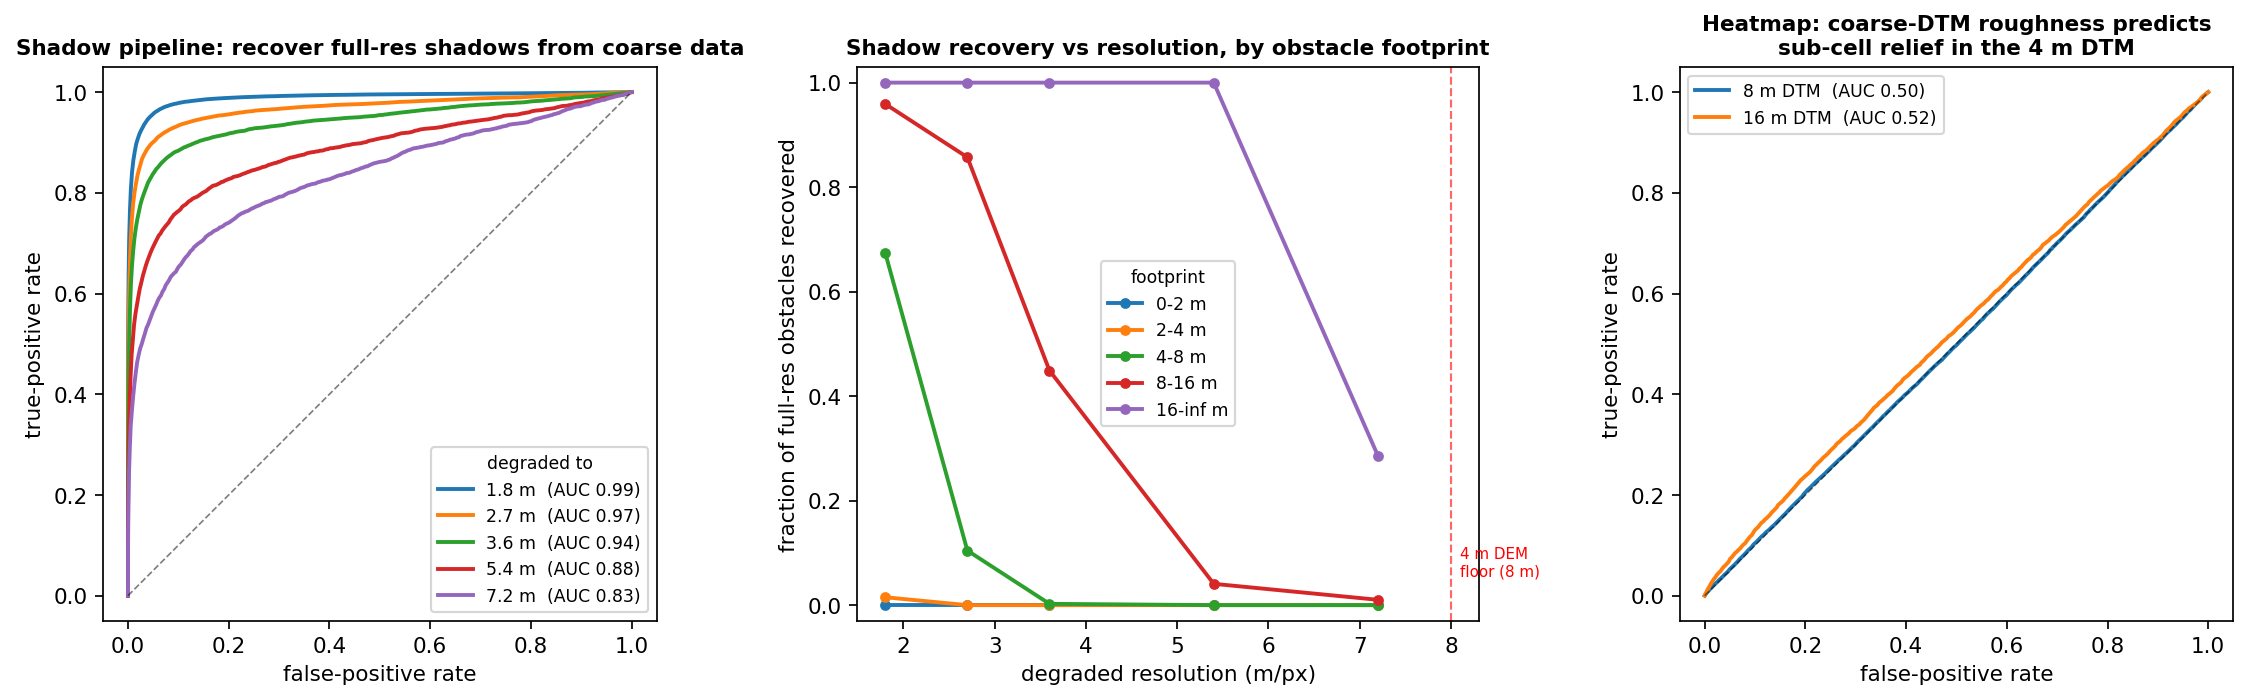
\includegraphics[width=\linewidth]{validation_curves}
\caption{Shadow-channel validation. Left: detection ROC at each degraded resolution.
Centre: the reach curve --- fraction of full-resolution obstacles recovered versus
resolution, by footprint. Right: the first, naive heatmap test, sitting on the chance
diagonal (an information boundary, not a fault).}
\label{fig:valcurves}
\end{figure}

\begin{figure}[t]
\centering
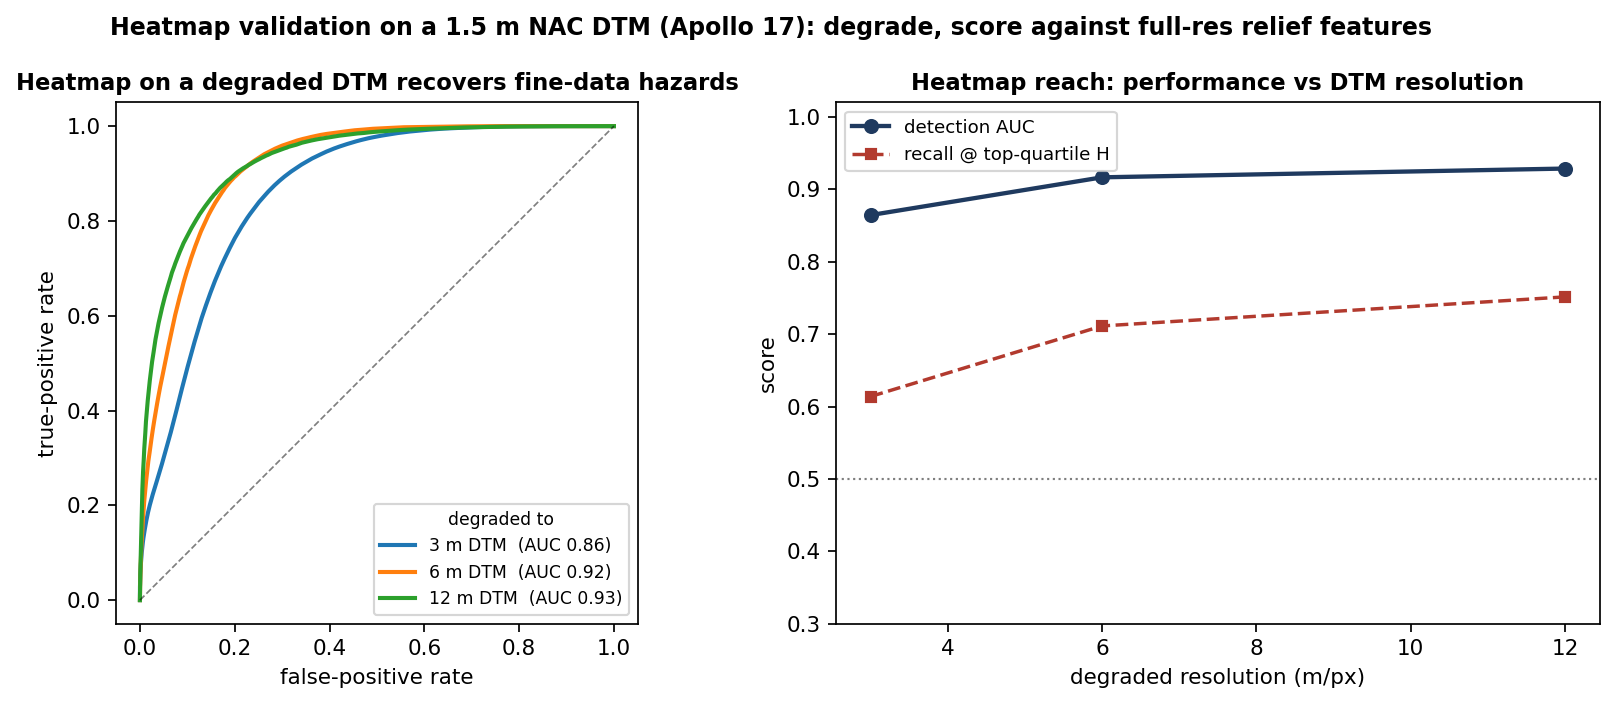
\includegraphics[width=0.92\linewidth]{heatmap_validation}
\caption{Heatmap validation done properly, on a \SI{1.5}{m} NAC DTM (Apollo~17): degrade
the model, score the coarse heatmap against the relief features the fine model resolves.
Detection AUC $0.86$--$0.93$ across $3$--\SI{12}{m}.}
\label{fig:valheat}
\end{figure}

\begin{figure}[t]
\centering
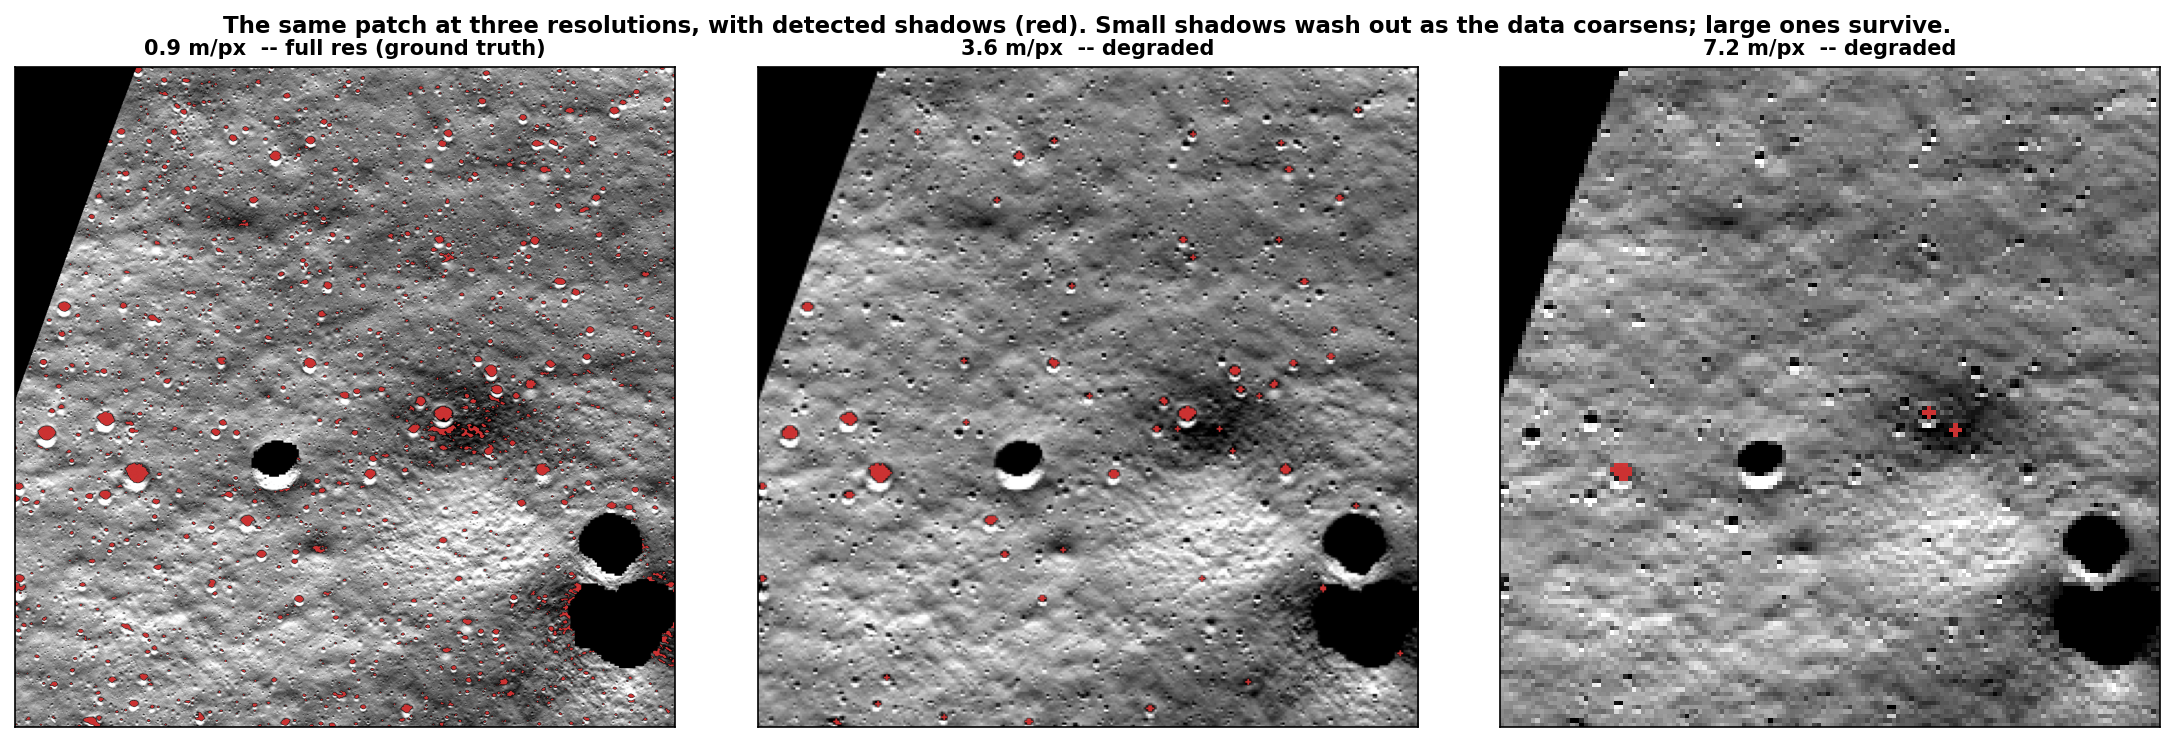
\includegraphics[width=\linewidth]{validation_ladder}
\caption{The same patch at \SI{0.9}{}, \SI{3.6}{}, and \SI{7.2}{\meter\per\px}, with
detected shadows in red. Small shadows wash out as the data coarsens; large ones survive
--- the reach curve made visible.}
\label{fig:valladder}
\end{figure}

\begin{limitbox}
Both ladders degrade single sites rather than using a genuinely different coarser sensor
(which would add its own noise), and the heatmap test runs on the scene where the
pipeline's scale settings were first shown (the weights are literature-fixed, so nothing
is fitted, but an independent site would harden it). A smooth-mare control is still owed,
to measure false alarms on benign ground. What stands: each channel has been handed worse
data and measured against the truth in better data, and each does the job it claims, with
a number attached.
\end{limitbox}

% =====================================================================
\section{Scrutiny: where a hostile reviewer would push}

\begin{description}[leftmargin=0pt,style=unboxed,itemsep=3pt]
\item[``96th percentile of a terrible neighbourhood is not an absolute hazard.'']
Correct, and the biggest limitation. $H$ is a within-scene ranking; the fix is a safe
control site (\cref{sec:future}). The relative claim stands; the absolute one waits.
\item[``You tried five settings; that is fishing.''] All five are reported, including
the one that fails outright. The flag holds from the 93rd to the 97th percentile
across every computable setting, on literature weights not tuned to Athena.
\item[``$n=1$, no controls.''] The counterfactual is one site --- but detection
performance is now measured directly by the resolution-ladder validation
(\cref{sec:validation}), independent of the Athena site. What one site still leaves open
is false-alarm behaviour on benign ground, which the mare control will supply.
\item[``Fine-scale roughness on a stereo model might be matching noise.''] The sharp
one: a stereo model has correlated error at the few-pixel scale, exactly where the flag
leans. Checked (\cref{sec:future}): the product confidence map \autocite{henriksen2017}
puts the touchdown at the maximum confidence value (14 of 14), level with the
safe-reference patch and about \SI{98.5}{\percent} of the valid DEM, so the flag is not
sitting in a poorly-correlated patch. That confidence code is coarse and near-saturated,
so it excludes a gross mismatch rather than bounding fine vertical precision; the clean,
stereo-free confirmation is multi-angle shadow relief (\cref{sec:future}).
\item[``Circularity.''] I knew the site failed. The guardrails keep the
\emph{measurement} clean, but the \emph{site selection} is hindsight, which is why
this is framed as detectability, not prediction.
\end{description}

% =====================================================================
\section{Future work, and why each step matters}
\label{sec:future}

\subsubsection{Control 1: safe-ground baseline \textemdash{} in-scene done, external mare next}
The in-scene form of this control is already run (\cref{sec:control}): it names the
channels that separate the hazard from the smoothest nearby ground. What it cannot give
is the \emph{absolute} safe floor, because the reference is the smoothest highland
patch, not a mare. The external mare control is the next step, and the trap to avoid is
the one \cref{sec:control} sidesteps: it must match the \SI{4}{\meter\per\px} resolution
and compare raw (or commonly-normalised) values, never per-scene $z$, since roughness is
scale-dependent \autocite{caifa2020} and $z$ is scene-relative. Done that way,
safe-ground values far below the touchdown's would turn ``rougher than
\SI{96}{\percent} of Mons Mouton'' into ``objectively unsafe.''

\subsubsection{Control 2: the stereo-confidence check \textemdash{} done}
Run. The \texttt{NAC\_DTM\_NOBILE03\_CONF} map \autocite{henriksen2017} puts the
touchdown at the maximum confidence (14 of 14), the same value as the safe-reference
patch and about \SI{98.5}{\percent} of the valid DEM, so the fine-scale roughness is
not a low-confidence artifact. The remaining caveat is that the code is coarse and
near-saturated: it excludes a gross stereo mismatch but does not bound fine vertical
precision, which is why the stereo-free cross-check below matters.

\subsubsection{Multi-angle shadow relief (Channel 2++)}
A single image gives obstacle footprints but needs an assumed sun elevation for height.
Two or more NAC frames of the site at different solar geometry let the heights be solved
directly (the geometry is known per frame from SPICE) and cross-checked: a real cast
shadow rotates and lengthens predictably as the sun moves, while noise and albedo do
not. It is \emph{stereo-independent}, so it is the natural confirmation of the
confidence caveat in Control~2, and the multi-angle stack it needs is the same data a
native-resolution $\bar\theta$ channel would require.

\subsubsection{A native-resolution $\bar\theta$ channel}
The existing $\bar\theta$ maps are too coarse (\cref{fig:bands}) to help at a landing
site. Fitting $\bar\theta$ from multi-angle NAC photometry would add an independent
sub-pixel channel, the one band the current two miss.

\subsubsection{Coupling to terrain-relative navigation}
A hazard map only matters if a lander can act on it. The end goal is to feed $H$ and
the obstacle census into the terrain-relative navigation loop as a landing-site
selection prior, so the descent avoids the worst few percent rather than reading it
in hindsight.

% =====================================================================
\section{Reproduce it exactly}

All paths under \texttt{HATI V2.0/}. Inputs: \texttt{data/athena/NAC\_DTM\_NOBILE03.TIF}
(\SI{4}{\meter\per\px}) and \texttt{...\_M1101075756\_90CM.IMG} (\SI{0.9}{\meter\per\px}).
Code: \texttt{scripts/athena\_counterfactual.py} (both channels),
\texttt{scripts/athena\_figure.py} (\cref{fig:money}),
\texttt{scripts/athena\_channel\_influence.py} (\cref{tab:influence}, \cref{fig:influence}),
and \texttt{scripts/athena\_safe\_control.py} (\cref{fig:control}).
Run \texttt{python scripts/athena\_counterfactual.py -{}-stage both}, then the
figure scripts. The validation (\cref{sec:validation}) is
\texttt{scripts/athena\_resolution\_validation.py} (shadow ladder) and
\texttt{scripts/heatmap\_resolution\_validation.py} (heatmap ladder, on the
\SI{1.5}{m} Apollo~17 DTM). Fixed constants (no per-run tuning): touchdown \ang{84.7906}\,S,
\ang{29.1957}\,E; elevation pixel (1181, 387); photo pixel (5248, 1721); MDS weight
ladder $1.0/0.9/0.8/0.6$ by ascending size; bias $-1.0$; $z$-clip $\pm4$; shadow
threshold $0.5\times$ local median (\SI{40}{\meter} window); obstacle floor
\SI{8}{\meter}; density radius \SI{25}{\meter}.

% =====================================================================
\section{Conclusion}

Using maps that predate the landing by thirteen years, and untuned weights from the
roughness literature, HATI's first channel ranks the actual IM-2 Athena touchdown in
the worst few percent of an already-dangerous site, driven by fine-scale texture that
a slope check misses, and its second channel confirms a dense obstacle layer below
the planning model's resolution. The site was detectable. A within-scene safe-ground control already names the
discriminating channels; a resolution-matched mare baseline and a stereo-confidence
check would harden ``worst few percent here'' into ``objectively unsafe.'' A
resolution-ladder validation gives each channel its first measured detection numbers ---
the shadow census an AUC of $0.83$--$0.99$ with a quantified size-reach, the heatmap
$0.86$--$0.93$ recovering fine-data hazards from coarse elevation models --- moving HATI
from one compelling case to a method with performance attached. The result asks for
neither more nor less than it earns: a hazard read from old data, by geometry alone, at
the place a mission was lost.

% =====================================================================
\section*{Acknowledgements}
This analysis rests entirely on the public LROC NAC stereo product
\texttt{NAC\_DTM\_NOBILE03} produced by the LROC team at Arizona State University
\autocite{robinson2010}, and on the LROC team's published measurement of the crater at
the touchdown. No part of HATI is affiliated with or endorsed by those teams.

% =====================================================================
\appendix
\section{Symbols and definitions}
\small
\begin{tabular}{@{}ll@{}}
\toprule
Symbol & Meaning \\
\midrule
$z,\ z_{ij}$ & elevation model (DTM); height at row $i$, column $j$ \\
$s$ & ground sample distance (pixel size, metres) \\
$\nabla z$ & gradient of elevation; its magnitude is the slope \\
$\nabla^2 z$ & Laplacian (curvature): $+$ in a pit, $-$ on a peak \\
$\arctan\lVert\nabla z\rVert$ & slope-angle field \\
$C_k[z]$ & the $k$-th Tier-1 roughness channel (convolution / windowed statistic) \\
$g(x)=\log(1+x)$ & tail-compressing transform \\
$\operatorname{med},\ \operatorname{IQR}$ & median and interquartile range (robust spread) \\
$\zeta_k$ & channel $k$ after robust standardisation (a $z$-score) \\
$\mathbf{w},\ b$ & literature weight vector and bias \\
$\sigma(a)=1/(1+e^{-a})$ & logistic (sigmoid) link \\
$H(x)\in[0,1]$ & fused hazard score at location $x$ \\
$\phi_k=w_k\zeta_k/\lVert\mathbf{w}\rVert_1$ & channel $k$'s additive contribution to the score \\
$h=L\tan e$ & obstacle height from shadow length $L$, sun elevation $e$ \\
$\lambda_{\min}=2s$ & resolution floor (Nyquist) \\
AUC & area under the ROC curve; $0.5$ is chance, $1$ perfect \\
\bottomrule
\end{tabular}

\medskip\noindent
The complete elevation pipeline, end to end:
\[
H(x)=\sigma\!\left(b+\frac{1}{\lVert\mathbf{w}\rVert_1}\sum_{k=1}^{10} w_k\,
\operatorname{clip}_{\pm c}\!\left[\frac{g(C_k[z])(x)-\operatorname{med}\,g(C_k[z])}{\operatorname{IQR}\,g(C_k[z])/1.349}\right]\right).
\]
Full derivations of every operator are in the companion \texttt{hati\_math.pdf}; a
ground-up tutorial that assumes only school mathematics is \texttt{hati\_textbook.pdf}.

\printbibliography[heading=bibintoc,title={References}]

\end{document}
